\documentclass[12pt,a4paper, twoside]{book}

\newcommand\studenta{Nguyễn Tất Đạt}
\newcommand\mssva{1610658}
\newcommand\studentb{Võ Hoàng Thành}
\newcommand\mssvb{1613206}
\newcommand\thesisname{Áp dụng phương pháp mạng nơ-ron nhân tạo để thiết kế bộ cân bằng hệ thống MIMO-VLC}
\newcommand\reportname{Luận văn tốt nghiệp đại học}
\newcommand\supervisor{TS. Phạm Quang Thái}
\newcommand\ngaygiaonhiemvu{24-9-2020}
\newcommand\ngayxongnhiemvu{11-1-2021}
\newcommand\noidungnhiemvu{
	\begin{itemize}\setlength\itemsep{-0.2em}
	\item Nhiệm vụ 1: Thiết lập hệ thống MIMO và lấy dữ liệu
	\item Nhiệm vụ 2: Xử lý dữ liệu thu được và đưa vào mạng nơ-ron nhân tạo để xử lý
	\item Nhiệm vụ 3: So sánh các kết quả thu được và nhận xét về tính hiệu quả của mạng nơ-ron nhân tạo
	\end{itemize}}


\usepackage[utf8]{vietnam}
\usepackage{titlesec} 
\usepackage{geometry}
\usepackage{amsmath}
\usepackage{graphicx}
\graphicspath{{./figure/}}
\usepackage{hyperref}

\hypersetup{
	colorlinks,
	citecolor=black,
	filecolor=black,
	linkcolor=black,
	urlcolor=black
}
\newtheorem{exam}{Ví dụ}[section]
\usepackage{acro}
\usepackage{cite}
\def\BibTeX{{\rm B\kern-.05em{\sc i\kern-.025em b}\kern-.08em
    T\kern-.1667em\lower.7ex\hbox{E}\kern-.125emX}}
\usepackage{listings}
\usepackage{fancyhdr}
\usepackage{tikz}
	\usetikzlibrary{shapes.geometric, arrows}
	\tikzstyle{startstop} = [rectangle, rounded corners, minimum width=2.5cm, minimum height=0.75cm,text centered, draw=black]
	\tikzstyle{io} = [trapezium, trapezium left angle=70, trapezium right angle=110, minimum width=2.5cm, minimum height=0.75cm, text centered, draw=black, text width=2cm]
	\tikzstyle{process} = [rectangle, minimum width=2.5cm, minimum height=0.75cm, text centered, draw=black, text width=3cm]
	\tikzstyle{decision} = [diamond, minimum width=2cm, minimum height=2cm, text centered, draw=black, text width=1cm]
	\tikzstyle{arrow} = [thick,->,>=stealth]


\geometry{
	a4paper,
	total={160mm,247mm},
	left=25mm,
	right=25mm,
	top=25mm,
	bottom=25mm,
}

	
\def\coverpage
	{
	\pagestyle{empty} 
	 	\begin{minipage}[b][25.5cm][t]{15cm}	
		\begin{center}
		{
		\vspace{3cm}
		\fontsize{20}{1}\selectfont 
		\textbf{\parbox[c][3cm]{14cm}{\centering \MakeUppercase{\thesisname}}
		}
		\\
		\vspace{0.1\paperheight}
		{\fontsize{14}{1}\selectfont 
		\MakeUppercase{\reportname}
		\\
		\vspace{0.05\paperheight}
		\studenta \space -- \mssva
		\\
		\studentb \space -- \mssvb \\
		Giảng viên hướng dẫn
		\\
		\supervisor
		}
		}
		\\
		\vspace{0.25\paperheight}
		\begin{minipage}{0.8\textwidth}
			\begin{minipage}{0.2\textwidth}
				
\includegraphics[width=0.7\linewidth]{hcmut_logo.jpg}
			\end{minipage}
			\begin{minipage}{\textwidth}\centering \raggedright
				{\fontsize{12}{1}\selectfont
				ĐẠI HỌC QUỐC GIA THÀNH PHỐ HỒ CHÍ MINH\\
				TRƯỜNG ĐẠI HỌC BÁCH KHOA\\
				KHOA ĐIỆN – ĐIỆN TỬ, BỘ MÔN VIỄN THÔNG\\
				}
			\end{minipage}
		\end{minipage}
		\\
		\vspace{0.05\paperheight}
		\the\month\space -- \the\year	
		\end{center}		
	\end{minipage}
	}
	
\def\nhiemvuluanvanpage	
{
	\cleardoublepage
	\begin{minipage}{0.5\textwidth}
		\begin{center}
			{\fontsize{9}{1}\selectfont
			ĐẠI HỌC QUỐC GIA THÀNH PHỐ HỒ CHÍ MINH\\
			TRƯỜNG ĐẠI HỌC BÁCH KHOA\\}
		\end{center}
	\end{minipage}
	\begin{minipage}{0.5\textwidth}
		\small
		\begin{center}
			{\fontsize{9}{1}\selectfont
			CỘNG HÒA XÃ HỘI CHỦ NGHĨA VIỆT NAM\\
			Độc lập -- Tự do -- Hạnh Phúc\\}
		\end{center}
	\end{minipage}
	\begin{center}
		\underline{\hspace{0.8\textwidth}}
	\end{center}

	\begin{minipage}{0.8\textwidth}
		Số:\underline{\hspace{2.4cm}}/BKĐT\\
		Khoa: \textbf{Điện -- Điện tử}\\
		Bộ môn: \textbf{Viễn thông}
	\end{minipage}
	\begin{center}
		\bfseries{\MakeUppercase{Nhiệm vụ luận văn tốt nghiệp}}
	\end{center}
	\begin{enumerate}\setlength\itemsep{-0.2em}
	\item 
	\begin{tabbing}
	Họ và tên: \= \studenta, \hspace{0.15\paperwidth} \= MSSV: \mssva 
	 \\ \> \studentb, \> MSSV: \mssvb
	\end{tabbing}
	\item Ngành: Điện -- Điện tử, Chuyên ngành: Kỹ thuật Điện tử -- Truyền thông
	\item Đề tài: \thesisname
	\item Nhiệm vụ: \noidungnhiemvu
	\item Ngày giao nhiệm vụ: \ngaygiaonhiemvu
	\item Ngày hoàn thành nhiệm vụ: \ngayxongnhiemvu
	\item 
	\begin{tabbing}
	Họ và tên người hướng dẫn: \hspace{0.25\paperwidth} \=  Phần hướng dẫn:\\
	\supervisor \> 100\%\\
	BM Viễn Thông, Khoa Điện – Điện Tử
	\end{tabbing}
	\end{enumerate}
	
	Nội dung và yêu cầu LVTN đã được thông qua Bộ Môn.
	
	\vspace{\baselineskip}
	\begin{minipage}{0.5\textwidth}
		\begin{center}
			{\fontsize{12}{1}\selectfont
			Tp. HCM, Ngày \underline{\hspace{0.5cm}} tháng \underline{\hspace{0.5cm}} năm 20\underline{\hspace{0.5cm}} \\
			\textbf{CHỦ NHIỆM BỘ MÔN}\\
			\par
			\vspace{0.06\paperheight}	
			PGS. TS. Hà Hoàng Kha
			}
		\end{center}
	\end{minipage}	
	\begin{minipage}{0.5\textwidth}
		\begin{center}
			{\fontsize{12}{1}\selectfont
			Tp. HCM, Ngày \underline{\hspace{0.5cm}} tháng \underline{\hspace{0.5cm}} năm 20\underline{\hspace{0.5cm}} \\
			\textbf{NGƯỜI HƯỚNG DẪN CHÍNH}\\
			\vspace{0.06\paperheight}	
			\supervisor
			}
		\end{center}
	\end{minipage}
	
	\vspace{\baselineskip}
	\begin{minipage}{0.8\textwidth}
		\textbf{PHẦN DÀNH CHO KHOA, BỘ MÔN:}\\
		Người duyệt (chấm sơ bộ): \underline{\hspace{3.5cm}} \\
		Đơn vị:\underline{\hspace{7.1cm}} \\
		Ngày bảo vệ:\underline{\hspace{6.1cm}}\\
		Điểm tổng kết:\underline{\hspace{5.75cm}}\\
		Nơi lưu trữ luận văn:\underline{\hspace{4.65cm}}\\
	\end{minipage}
}

\DeclareAcronym{snr}{
short = SNR,
long = Signal to Noise Ratio
}

\DeclareAcronym{ann}{
short = ANN,
long = Artificial Neural Networks
}

\DeclareAcronym{mimo}{
short = MIMO ,
long = Multiple-input Multiple-output
}

\DeclareAcronym{vlc}{
short = VLC,
long = Visible Light Communication
}

\DeclareAcronym{ieee}{
short = IEEE,
long = Institute of Electrical and Electronics Engineers
}
\DeclareAcronym{oled}{
	short = OLED,
	long = organic light-emitting diode
}
\DeclareAcronym{owc}{
	short = OWC,
	long = Optical wireless communication
}
\DeclareAcronym{pnn}{
	short = PNN,
	long = Probabilistic neural network
}
\DeclareAcronym{ber}{
	short = BER,
	long = Bit error rate
}
\DeclareAcronym{nrz}{
	short = NRZ,
	long = None Return to Zero 
}
\DeclareAcronym{pdf}{
	short = PDF,
	long = Probability Distribution Function 
}

\DeclareAcronym{fov}{
	short = FOV,
	long = Field Of View 
}

\DeclareAcronym{rz}{
	short = RZ,
	long = Return to Zero
}

\DeclareAcronym{los}{
	short = LOS,
	long = Light Of Sight
}

		
\begin{document}

\coverpage

\nhiemvuluanvanpage
		
\frontmatter

\titleformat{\chapter}
  {\Large\bfseries}
  {\thechapter .}
  {.5em}
  {\filleft\MakeUppercase}
  [\vspace{.5ex}]

\chapter*{Lời cám ơn}
	

\vspace{\baselineskip}
Đầu tiên, chúng em xin được gửi lời cảm ơn chân thành đến thầy hướng dẫn luận văn của mình TS.Phạm Quang Thái. Trong quá trình thực hiện luận văn, thầy là người đã nhiệt tình hỗ trợ, chỉ dẫn giúp chúng em củng cố kiến thức đồng thời chỉ ra những vấn đề cốt lõi giúp  chúng em có định hướng đúng đắn để hoàn thành luận văn.
\vspace{\baselineskip}

Tiếp đến, chúng em xin được gửi lời cảm ơn đến các thầy cô đã và đang dạy tại trường Đại Học Bách Khoa Tp.HCM và đặc biệt là các thầy cô ở Bộ Môn Viễn Thông đã giúp chúng em xây dựng được kiến thức nền tảng, là cơ sở để chúng tôi thực hiện được luận văn này.
\vspace{\baselineskip}

Cuối cùng chúng em xin gửi lời cảm ơn đến gia đình, bạn bè, đồng nghiệp đã hết sức giúp đỡ, quan tâm, động viên để chúng tôi có điều kiện thuận lợi để thực hiện luận văn này.
\vspace{\baselineskip}


Xin chân thành cảm ơn!


	\vspace{\baselineskip}
	\hfill
	\begin{minipage}{0.5\textwidth}
		\begin{center}
			{\fontsize{12}{1}\selectfont
			Tp. HCM, \today 
			\vspace{0.1\paperheight}	
			\studenta
			,\space \studentb
			}
		\end{center}
	\end{minipage}
	
\chapter*{Lời cam đoan}
	Tôi tên: \studenta \space (MSSV: \mssva), 
	\studentb \space (MSSV: \mssvb),
	là sinh viên chuyên ngành Kỹ thuật Điện tử - Truyền thông, tại Trường Đại học Bách Khoa, Đại học Quốc gia thành phố Hồ Chí Minh. Chúng tôi xin cam đoan những nội dung sau đều là sự thật: 
	
	\begin{itemize}
		\item  Công trình nghiên cứu này hoàn toàn do chính chúng tôi thực hiện; 
		\item  Các tài liệu và trích dẫn trong luận văn này được tham khảo từ các nguồn thực tế, có uy tín và độ chính xác cao; 
		\item  Các số liệu và kết quả của công trình này được chúng tôi tự thực hiện một cách độc lập và trung thực.
	\end{itemize}

	\vspace{\baselineskip}
	\hfill
	\begin{minipage}{0.5\textwidth}
		\begin{center}
			{\fontsize{12}{1}\selectfont
			Tp. HCM, \today 
			\vspace{0.1\paperheight}	
			\studenta 
			,\space \studentb
			}
		\end{center}
	\end{minipage}

\chapter*{Tóm tắt nội dung}
	\vspace{\baselineskip}
\textbf{Bài toán nghiên cứu:}

Sử dụng kết quả đo đạc thực tế của hệ thống MIMO-VLC sử dụng đèn OLED để xây dựng mạng nơ-ron xác suất nhằm khôi phục tín hiệu sau khi đi qua kênh truyền.

\vspace{\baselineskip}

\textbf{Phương pháp tiếp cận:}

Dùng phần mềm Matlab để tạo tín hiệu NRZ điều khiển 2 đèn OLED trong phòng thí nghiệm. Sau khi đi qua hệ thống thực tế tín hiệu thu được sẽ được xử lý qua Matlab để phục vụ cho việc khảo sát mạng nơ-ron xác suất. Thông số tỉ lệ lỗi bit sẽ được đem ra để đánh giá khả năng của mạng nơ-ron trong hệ thống MIMO-VLC. 

\vspace{\baselineskip}


\textbf{Kết quả:}

\vspace{\baselineskip}
\textbf{Kết luận:}




\chapter*{Abstract}
	\vspace{\baselineskip}
\textbf{Research problem:}

Using neural network to enhance the demodulation of MIMO-VLC system .
\vspace{\baselineskip}

\textbf{Research methods:}

Using Matlab to create NRZ signal to control 2 OLED in labortary. After transmitting through a real system, received signal is analysised using Matlab to put in a neural network. Bit error rate will be compared to evaluate the efficiency of neural network in MIMO-VLC system.
\vspace{\baselineskip}

\textbf{Result:}
\vspace{\baselineskip}

\textbf{Conclusion:}


\tableofcontents
{%
 \let\oldnumberline\numberline%
 \renewcommand{\numberline}{\figurename~\oldnumberline}%
 \listoffigures%
}
{%
\let\oldnumberline\numberline%
\renewcommand{\numberline}{\tablename~\oldnumberline}%
\listoftables%
}
\printacronyms[name = {Danh sách từ viết tắt}]
	
\mainmatter

\fancyhead{}  % Clears all page headers and footers
\fancyhead[L]{\nouppercase\leftmark}
\fancyhead[R]{\thepage}
\cfoot{}
\pagestyle{fancy}

\titleformat{\chapter}
  {\Large\bfseries}
  {Chương \thechapter .}
  {.5em}
  {\filleft\MakeUppercase}
  [\vspace{.5ex}]

\chapter{Giới thiệu} \label{sec:chuong-1} % câu lệnh này nghĩa là bắt đầu một chương với tên gọi là Giới thiệu, chương này được đánh nhãn là sec:chuong-1 để có thể liên kết đến nếu cần thiết

\section{Đặt vấn đề} \label{sec:chuong-1-datvande}
 % câu lệnh này nghĩa là bắt đầu mục nhỏ cấp 1 trong chương hiện tại
Trên thế giới ngày nay, truyền tín hiệu bằng ánh sáng khả kiến \ac{vlc} đang rất được quan tâm bởi các nhà nghiên cứu cũng như kĩ sư bởi tính tiện dụng của nó. Tuy chưa được áp dụng rộng rãi, đại trà như công nghệ này rất có tiềm năng trong tương lai. Hàng trăm bài báo, video bạn có thể kiếm được trên internet nói về chủ đề này.Là những sinh viên chúng em cũng muốn tiếp cận những kiến thức mới, công nghệ mới. Việc khảo sát về hoạt động của hệ thống \ac{vlc} trong phòng thí nghiệm cũng như mô phỏng đã đươc các anh chị khoá trước trình bày khá rỏ ràng, nhưng hệ thống chỉ có 1 đèn và 1 bộ thu. TRong luận văn này,chúng em sẽ làm thí nghiệm về hệ thống VLC sử dụng 2 đèn và 1 bộ thu, mô phòng gần giống với thực tế. Ngoài ra, việc sử dụng mạng nơ-ron nhân tạo để thiết kế bộ cân bằng cho hệ thống VLC cũng được nghiên cứu khá nhiều nên tụi em cũng sử dụng mạng nơ-ron xác suất để khảo sát xem nó có hoạt động tốt trong hệ thống MIMO-VLC không.  



Câu hỏi nghiên cứu đặt ra của luận văn là:
\begin{itemize}
	\item Việc sử mạng nơ-ron xác suất có hiệu quả trong việc làm bộ cân bằng cho hệ thống MIMO-VLC.
	\item Tốc độ bit bằn bao nhiêu thì mạng nơ-ron xác suất sẽ cho ra tỉ lệ lỗi bit không còn đạt ngưỡng.
	\item Khoảng cách tối đa là bao nhiêu thì mạng nơ-ron sẽ không còn cân bằng chính xác với điều kiện trong phòng thí nghiệm.  
	
\end{itemize}




	Trong chương 2, cơ sở lý thyết về MIMO-VLC, line coding và neural network sẽ được trình bày. 
	Trong chương 3, các kết quả mô phỏng sẽ được so sánh và phân tích. 
	Cuối cùng, chương 4 đưa ra kết luận chung.

\section{Phạm vi và phương pháp nghiên cứu}


\begin{itemize}
	\item  Sinh viên thực hiện đo đạc trong phòng thí nghiệm ở trường, các thiết bị trong phòng thí nghiệm do thầy hướng dẫn cung cấp. Do kích thước phòng có hạn nên chúng em chỉ khảo sát ở khoảng cách lớn nhất là 2m.
	\item  Khảo sát sự thay đổi của tỉ lệ lỗi bit theo tốc độ bit và sự thay đổi của tỉ lệ lỗi bit theo khoảng cách. 
	\item Tín hiệu thí nghiệm là tín hiệu NRZ được tạo từ code Matlab, sẽ được truyền đi qua hệ thống thực tế.  
	\item Mạng nơ-ron nhân tạo được sử dụng là mạng nơ-ron xác suất \ac{pnn}, mạng này có sẵn trong Matlab nên rất thuận tiện cho việc khảo sát.
	
\end{itemize}
	
	
	
	
\section{Các đóng góp của luận văn}
	
Luận văn này có các đóng góp như sau:

\begin{itemize}
	\item Hiện thực hoá bộ cân bằng tín hiệu dùng phương pháp mạng nơ-ron nhân tạo, cụ thể là \ac{pnn} dùng phần mềm Matlab.
	\item Đưa ra được các số liệu về tỉ lệ lỗi bit sát với lý thuyết. Các số liệu này cũng có thể đem khảo sát ở thực tế.
	\item So sánh và phân tích \ac{ber} trên các tốc độ bit và khoảng cách.
\end{itemize}	
\chapter{Cơ sở lý thuyết} \label{sec:chuong-2}

\section{Line coding}

Trong viễn thông, mã đường truyền hay còn được gọi là điều chế số dải nền là một mã được chọn để sử
dụng cho việc truyền nhận của tín hiệu trong hệ thống, mã đường truyền thường được sử dụng trong truyền thông
tin số. Hay nói cách khác, nó dùng để ánh xạ chuỗi dữ liệu của chúng ta thành một dạng tín hiệu mà có thể truyền
nhận được.

\vspace{\baselineskip}
Mã đường truyền biểu diễn tín hiệu số (chuỗi nhị phân) được truyền đi, bằng một dạng sóng được đặc trưng
bởi một đặc tính nào đó của kênh truyền vật lý, hoặc thiết bị thu như là điện áp, dòng điện, photon. Có ba loại chính
trong mã hóa đường truyền, đó là Unipolar, Bi-Polar, Polar.

\begin{figure} [ht]
	\begin{center}
		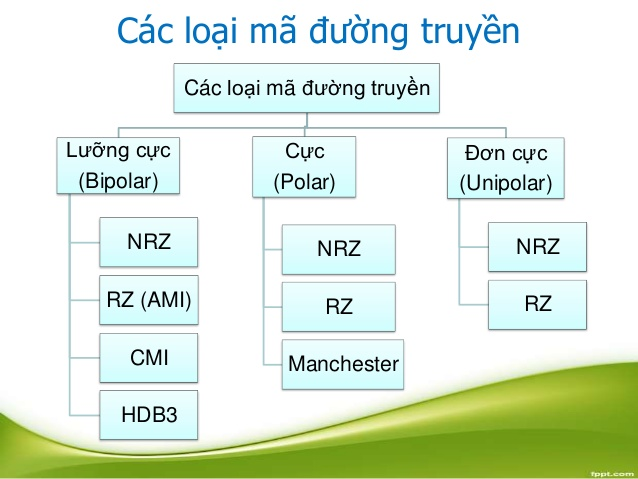
\includegraphics[width=0.75\textwidth,keepaspectratio]
		{linecoding.jpg}
	\end{center}
	\caption{Các loại mã đường truyền} 
	 
\end{figure}

Mục đích của mã hoá đường truyền là \cite{linecoding}:

\begin{itemize}
	\item Tạo ra phổ tín hiệu sao cho phù hợp với kênh truyền.
	\item Tạo khả năng tách tín hiệu đồng bộ ở bộ thu.
	\item Tăng tốc độ truyề dẫn.
	\item Tạo khả năng phát hiện và sửa lỗi.  
\end{itemize}

Từ những mục đích đó, một số yếu tố cũng được đề ra để giúp người thiết kế có thể chọn lựa mã đường
truyền phù hợp cho hệ thống, khi chọn lựa mã đường truyền, ta phải lưu tâm đến những yếu tố \cite{linecoding}:

\begin{itemize}
	\item Thành phần một chiều DC, băng thông của hệ thống.
	\item Tỷ lệ lỗi, khả năng tự phát hiện lỗi.
	\item Đơn giản trong việc mã hóa và giải mã.
	\item  Khả năng khôi phục xung clock.
\end{itemize}	

\subsection{None return to Zero}

Trong hệ thống viễn thông, NRZ là mã đường truyền nhị phân, mà trong đó các bit 1 được đại diện bởi một
giá trị, thông thường là điện áp dương, trong khi đó các bit 0 được dại diện với một giá trị khác, thông thường là
điện áp âm. Bản thân NRZ vốn không có khả năng tự đồng bộ xung clock, nên một số kỹ thuật đồng bộ khác phải
được đưa vào để tránh sự trượt bit. Với một tốc độ bit nhất định, NRZ chỉ cần một nửa băng thông dải nền so với
mã manchester. Có ba loại mã hóa NRZ: bi-polar, polar, unipolar.


  
	\subsubsection{Uni-polar NRZ}
	
	Trong hệ thống viễn thông, \ac{nrz} là mã đường truyền nhị phân, mà trong đó các bit 1 được đại diện bởi một
	giá trị, thông thường là điện áp dương, trong khi đó các bit 0 được dại diện với một giá trị khác, thông thường là
	điện áp âm. Bản thân \ac{nrz} vốn không có khả năng tự đồng bộ xung clock, nên một số kỹ thuật đồng bộ khác phải
	được đưa vào để tránh sự trượt bit. Với một tốc độ bit nhất định, \ac{nrz} chỉ cần một nửa băng thông dải nền so với
	mã manchester. Có ba loại mã hóa NRZ: bi-polar, polar, unipolar.
	
	\vspace{\baselineskip}
	Trong NRZ đơn cực (Unipolar NRZ), bit 1 được đại diện bởi mức điện áp DC trên đường truyền, trong khi đó bit 0 là không
	có điện áp, hay còn gọi là mức điện áp 0V hoặc là đất. Vì lý do này, mã uni-polar NRZ còn được gọi là mã tắt mở
	(On-Off keying). Một điểm độc nhất của tín hiệu NRZ đơn cực chính là việc tồn tại mức DC trong quá trình truyền
	nhận, do đó phổ của tín hiệu tại tần số zero sẽ khác không. Việc này gây ra hai vấn đề chính: thứ nhất, công suất
	DC được truyền đi dẫn đến sự tiêu hao công suất hơn nhiều so với các phương pháp giải mã mà không có thành
	phần DC, và thứ hai, việc tồn tại thành phần DC buộc đường truyền phải được DC coupling \cite{linecoding}.
	
\begin{center}	
\begin{figure} [ht]
	\begin{center}
		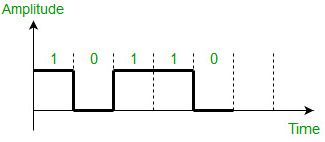
\includegraphics[width=0.65\textwidth,keepaspectratio]
		{Unipolarnrz.jpg}
	\end{center}
	\caption{Dạng tín hiệu mã Uni-Polar NRZ } 
	
\end{figure}
\end{center}

\begin{center}
	

\begin{figure} [ht]
	\begin{center}
		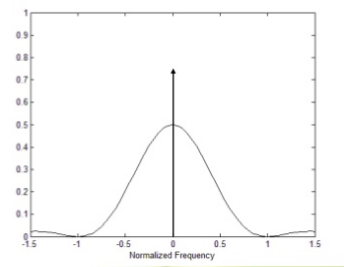
\includegraphics[width=0.5\textwidth,keepaspectratio]
		{pcsunrz.png}
	\end{center}
	\caption{Phổ công suất của tín hiệu NRZ đơn cực } 
	
\end{figure}
\end{center}

\vspace{\baselineskip}

\textbf{Uni-polar NRZ}
\begin{itemize}
	\item Ưu điểm: Đơn giản,  tiêu tốn ít băng thông.
	\item Nhược điểm: Có thành phần DC, không có khả năng sửa lỗi, khó khôi phục xung clock do không có
	hài tại tần số xung clock (f) nên khó đồng bộ, tồn tại chuỗi bit 0 dài trong dữ liệu làm mất tính đồng bộ.
\end{itemize}

\subsubsection{Polar NRZ}

Trong mã hóa NRZ lưỡng cực, bit 1 được đại diện bởi điện áp dương, bit 0 được đại diện bởi điện áp âm.
Trong mã này, mức điện áp tín hiệu sẽ được thay đổi từ dương sang âm tại cạnh xuống của chu kỳ xung clock trước.
Một ứng dụng phổ biến của mã này chính là chuẩn giao tiếp nối tiếp RS-232, trong đó mức 1 được đặc trưng bởi
điện áp trong khoảng -12V đến -5V và mức 0 được đặc trưng bởi điện áp trong khoảng 5V đến 12V. \ref{fig:pnrz} mô
tả dạng tín hiệu của mã hóa NRZ.

\begin{center}
	
	
	\begin{figure} [ht]
		\begin{center}
			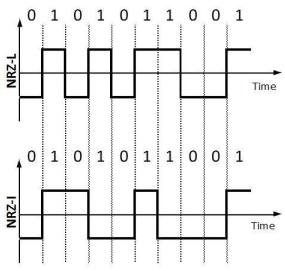
\includegraphics[width=0.5\textwidth,keepaspectratio]
			{polarnrz.png}
		\end{center}
		\caption{Dạng tín hiệu mã NRZ } 
		\label{fig:pnrz}
		
	\end{figure}
\end{center}

Polar NRZ còn thường được sử dụng dưới hai dạng mã hóa chính, đó chính là NRZ-I và NRZ-L như được
mô tả trong hình trên. Trong đó, NRZ-L đơn giản hơn, nhưng cần phân biệt cực tính của tín hiệu, trong khi đó
NRZ-I đáng tin cậy hơn, trong môi trường truyền có nhiều tạp âm, phát hiện sự chuyển mức tín hiệu dễ dàng hơn
là so sánh tín hiệu với một giá trị ngưỡng như trong NRZ-L.


\begin{center}
	
	
	\begin{figure} [ht]
		\begin{center}
			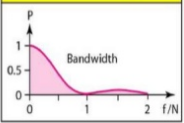
\includegraphics[width=0.5\textwidth,keepaspectratio]
			{phopnrz.png}
		\end{center}
		\caption{Phổ của tín hiệu Polar-NRZ } 
		
		
	\end{figure}
\end{center}

Nhận thấy phổ của tín hiệu NRZ trong trường hợp này giống như trong trường hợp uni-polar NRZ, do thực
chất hai trường hợp chỉ là kết quả quá trình DC-offset của nhau.

	\vspace{\baselineskip}
Nhận xét về mã polar-NRZ:

\begin{itemize}
	\item Ưu điểm: Đơn giản, dễ thiết kế, ít tiêu tốn băng thông
	\item Nhược điểm: Có thành phần DC, không có khả năng sửa lỗi, khó khôi phục xung clock do không có
	hài ở tần số f, ít được sử dụng cho việc truyền tín hiệu đi xa.
	
\end{itemize}

\subsubsection{Bi-polar NRZ}

Trong tín hiệu Bi-polar NRZ, bit 0 được đặc trưng bởi mức điện áp 0V, trong khi đó mức 1 được đặc trưng
bởi mức điện áp dương hoặc âm, luân phiên nhau.

\begin{center}
	
	
	\begin{figure} [ht]
		\begin{center}
			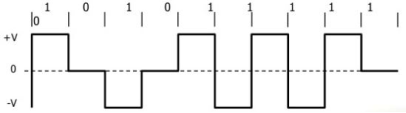
\includegraphics[width=0.75\textwidth,keepaspectratio]
			{bipolar.png}
		\end{center}
		\caption{Dạng tín hiệu Bi-polar NRZ } 
		
		
	\end{figure}
\end{center}

\begin{center}
	
	
	\begin{figure} [ht]
		\begin{center}
			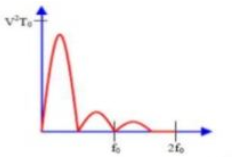
\includegraphics[width=0.5\textwidth,keepaspectratio]
			{phobipolar.png}
		\end{center}
		\caption{Dạng phổ của tín hiệu Bi-polar NRZ } 
		
		
	\end{figure}
\end{center}

Nhận xét về mã Bi-polar NRZ:

\begin{itemize}
	\item Ưu điểm: không có thành phần DC, tiêu tốn ít băng thông hơn so với Unipolar và polar NRZ, có khả
	năng phát hiện lỗi.
	\item Nhược điểm: không có thành phần xung clock để đồng bộ hóa.
	
\end{itemize}

\subsection{Return to Zero (RZ)}

\ac{rz} là tên gọi của loại mã hóa trong hệ thống viễn thông, mà trong đó mức tín hiệu rơi về vị trí 0V sau mỗi
chu kỳ xung. Khác với mã \ac{nrz}, \ac{rz} là tín hiệu có thể tự đồng bộ (self-clocking), do đó không cần một tín hiệu
xung clock riêng biệt gửi cùng với dữ liệu, nhưng bên cạnh đó phải sử dụng gấp đôi băng thông so với cùng một
tốc độ dữ liệu trong mã \ac{nrz}.

\subsubsection{Uni-polar RZ}


Cũng giống như uni-polar NRZ, tuy nhiên độ rộng xung chỉ bằng một nửa so với chu kỳ xung. Trong mã
này, bit 1 được đại diện bởi dạng sóng có mức điện áp chuyển từ cao sang thấp trong một chu kỳ xung, và bit 0
được đại diện bởi trạng thái nghỉ (mức thấp), dạng tín hiệu được mô tả như \ref{fig:uprz}.

\begin{center}
	
	
	\begin{figure} [ht]
		\begin{center}
			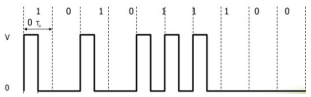
\includegraphics[width=0.75\textwidth,keepaspectratio]
			{Uprz.png}
		\end{center}
		\caption{Dạng tín hiệu của Uni-polar RZ }
		\label{fig:uprz} 
		
		
	\end{figure}
\end{center}

\begin{center}
	
	
	\begin{figure} [ht]
		\begin{center}
			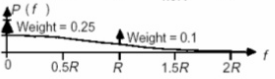
\includegraphics[width=0.5\textwidth,keepaspectratio]
			{phoUprz.png}
		\end{center}
		\caption{Dạng phổ của tín hiệu của Uni-polar RZ }
		 
		
		
	\end{figure}
\end{center}

Nhận xét về mã Uni-polar RZ:

\begin{itemize}
	\item Ưu điểm: đơn giản, xuất hiện hài tần số f, có thể dùng để khôi phục xung clock.
	\item Nhược điểm: tồn tại thành phần DC, không có khả năng sửa lỗi khi xuất hiện nhiễu, băng thông sử
	dụng gấp 2 lần so với unipolar NRZ.
\end{itemize}

\subsubsection{Polar RZ}

Trong mã hóa polar RZ, bit 1 được đặc trưng bởi dạng sóng có mức điện áp chuyển từ +V sang 0 trong một
chu kỳ xung, và bit 0 được đặc trưng bởi dạng sóng có mức điện áp chuyển từ -V sang 0 trong một chu kỳ xung,
dạng sóng này được mô tả trong \ref{fig:plprz} :

\begin{center}
	
	
	\begin{figure} [ht]
		\begin{center}
			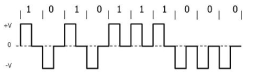
\includegraphics[width=0.75\textwidth,keepaspectratio]
			{Plrz.png}
		\end{center}
		\caption{Dạng tín hiệu của Polar RZ }
		\label{fig:plprz} 
		
		
	\end{figure}
\end{center}

\begin{center}
	
	
	\begin{figure} [ht]
		\begin{center}
			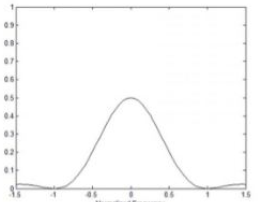
\includegraphics[width=0.5\textwidth,keepaspectratio]
			{phoPlrz.png}
		\end{center}
		\caption{Dạng phổ của tín hiệu của Polar RZ }
		
		
		
	\end{figure}
\end{center}

Nhận xét về mã Polar-RZ:

\begin{itemize}
	\item Ưu điểm: đơn giản, dễ thực hiện.
	\item Nhược điểm: có thành phần DC, không có khả năng sửa lỗi, không có thành phần clocking để đồng
	bộ hoá tuy nhiên xung clock có thể được khôi phục bằng cách chấn chỉnh các tín hiệu nhận được, chiếm gấp đôi
	băng thông so với polar NRZ.
\end{itemize}

\subsubsection{Bi-polar RZ}

Trong tín hiệu Bi-polar RZ, bit 0 đặc trưng bởi điện áp 0V, mức 1 được luân phiên chuyển từ điện áp ±V
xuống 0 trong một chu kỳ xung.

\begin{center}
	
	
	\begin{figure} [ht]
		\begin{center}
			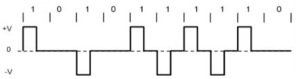
\includegraphics[width=0.75\textwidth,keepaspectratio]
			{biPlrz.png}
		\end{center}
		\caption{Dạng phổ của tín hiệu của Bi-polar RZ }
		
		
		
	\end{figure}
\end{center}

\begin{center}
	
	
	\begin{figure} [ht]
		\begin{center}
			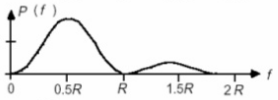
\includegraphics[width=0.75\textwidth,keepaspectratio]
			{phobiPlrz.png}
		\end{center}
		\caption{Dạng phổ của tín hiệu của Bi-polar RZ }
		
		
		
	\end{figure}
\end{center}

Nhận xét về mã hoá Bi-polar RZ:

\begin{itemize}
	\item Ưu điểm: không có thành phần DC, tiêu tốn ít băng thông hơn so với Unipolar và polar RZ, có khả
	năng phát hiện lỗi, clock có thể được tách ra từ cách chấn chỉnh các tín hiệu thu được.
	\item Nhược điểm: chưa khăc phục được tình trạng dữ liệu có nhiều bit 0 liên tiếp.
\end{itemize}

\section{Hệ thống MIMO-VLC}
\subsection{Tổng quan về VLC}
Ngày nay kết nối internet đã trở thành nhu cầu cơ bản của con người. Tuy nhiên, không dừng lại ở việc truy
cập internet, mà nhu cầu về tốc độ cũng không ngừng tăng cao.
\begin{center}
\begin{figure} [ht]
	\begin{center}
		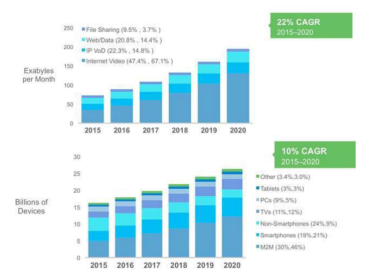
\includegraphics[width=0.5\textwidth,keepaspectratio]
		{luuluongthietbi.png}
	\end{center}
	\caption{Biểu đồ tăng trưởng lưu lượng và số lượng thiết bị } 
	
\end{figure}
\end{center}

Theo dự báo chỉ số tăng trưởng mạng (VNI) thường niên của cisco lần thứ 10, lưu lượng cũng như số lượng
thiết bị truy cập internet tăng với tốc độ chóng mặt trong những năm qua, thậm chí còn được cisco dự đoán sẽ tăng
với tốc độ cao hơn trong những năm tới. Một số lượng thiết bị và nhu cầu lưu lượng khổng lồ như vậy đòi hỏi một
băng thông cực lớn để truyền tải dữ liệu, công nghệ truyền không dây Wi-fi dần trở nên không đáp ứng được, do
đó không thể tránh khỏi việc nghiên cứu và đưa ra một công nghệ mới có thể đáp ứng được nhu cầu to lớn đó. Một
trong những công nghệ đã nhận được được sự quan tâm mạnh mẽ là truyền thông không dây quang \ac{owc}.

\vspace{\baselineskip}
\ac{owc} là ứng viên tiềm năng cho truyền dẫn không dây trong nhà (indoor). Kỹ thuật này sử dụng ánh sáng để truyền dẫn thông tin thay cho sóng điện tử (vốn đã hạn chế về băng thông). Do đó ánh sáng không thể xuyên qua vật thể nên sẽ không dây can nhiễu với các hệ thống khác và mang lại tính bảo mật cao. Hệ thống \ac{owc} có các ưu điểm như thiết lập nhanh, tốc độ truyền nhanh hơn so với các công nghệ truyền thông không dây hiện nay như Bluetooth, Wifi. Hơn nữa, việc sử dụng những linh kiện đơn giản với giá thành thấp như sử dụng \ac{oled} ở phía phát và photodetector ở phía thu, khiến cho việc sử dụng vào thực tế sẽ dễ dàng hơn. Với sự phát triển của công nghệ vật liệu, đặc biệt là sự phát triển không ngừng của \ac{oled} đã hướng sự quan tâm về việc nghiên cứu cũng như ứng dụng công nghệ truyền thông không dây sử dụng ánh sáng khả kiến \ac{vlc}. Đây được xem là một giải pháp khả thi cho truyền thông quang không dây trong tương lai \cite{vlc}.

\vspace{\baselineskip}
Giao tiếp ánh sáng khả kiến (VLC) là một biến thể truyền thông dữ liệu sử dụng ánh sáng nhìn thấy được giữa 400 và 800 THz (780–375 nm). VLC là một tập hợp con của các công nghệ truyền thông không dây quang học.

\begin{center}	
	\begin{figure} [ht]
		\begin{center}
			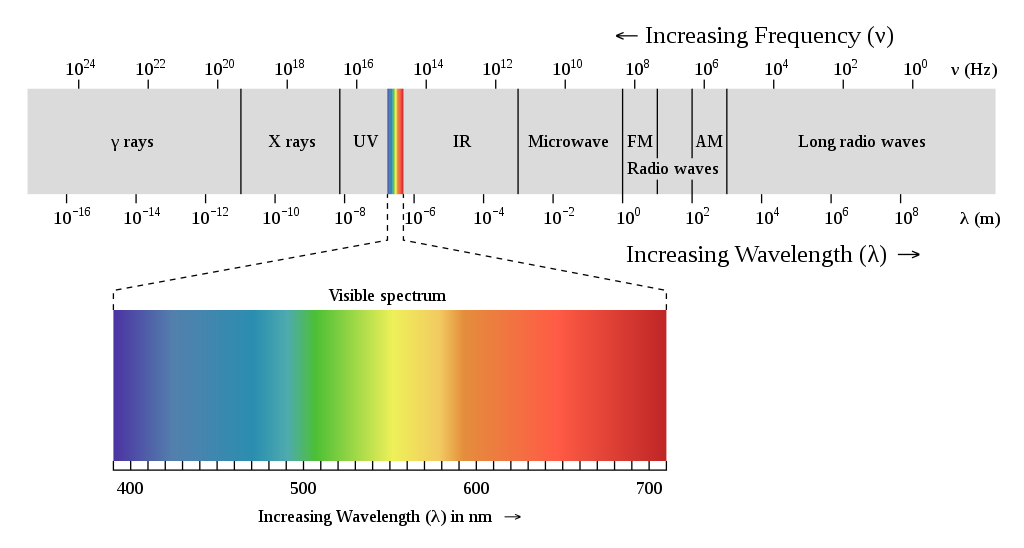
\includegraphics[width=0.75\textwidth,keepaspectratio]
			{vunganhsangkhakien.png}
		\end{center}
		\caption{Vùng ánh sáng khả kiến được sử dụng cho VLC } 
	\end{figure}
\end{center}

Công nghệ này sử dụng đèn huỳnh quang (đèn thông thường, không phải thiết bị liên lạc đặc biệt) để truyền tín hiệu ở tốc độ 10 kbit/s hoặc đèn LED lên đến 500 Mbit/s trong khoảng cách ngắn. 

\vspace{\baselineskip}
VLC có thể được sử dụng như một phương tiện truyền thông cho điện toán phổ biến, vì các thiết bị mang ánh sáng (như đèn trong nhà / ngoài trời, TV, biển báo giao thông, màn hình thương mại và đèn pha / đèn hậu xe hơi) được sử dụng ở mọi nơi. Sử dụng ánh sáng có thể nhìn thấy được cũng ít nguy hiểm hơn đối với các ứng dụng công suất cao vì con người có thể cảm nhận được nó và hành động để bảo vệ mắt khỏi bị hư hại \cite{askk}.

\begin{center}	
	\begin{figure} [ht]
		\begin{center}
			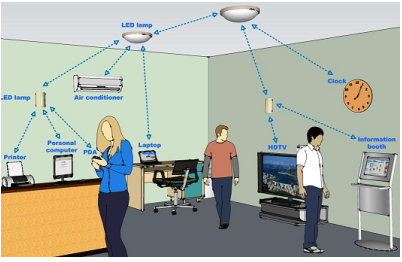
\includegraphics[width=0.75\textwidth,keepaspectratio]
			{futurevlc.png}
		\end{center}
		\caption{Công nghệ VLC trong tương lai } 
	\end{figure}
\end{center}


	

	
	
	\subsection{Phân loại kênh truyền}
	
Cấu hình đường truyền cho hệ thống \ac{vlc} dựa vào mức độ định hướng giữa bộ phát và bộ thu, do đó được chia thành ba loại: Trực tiếp (LOS-Line Of Sight), không trực tiếp (NLOS-directed Non Line Of Sigth) và Lai ghép (non-derected NLOS). Đường truyền trực tiếp (LOS) từ bộ phát và bộ thu có công suất cao nhất vì nó chịu suy hao nhỏ nhất từ ảnh hưởng từ môi trường. Đối
với đường truyền không trực tiếp, các thiết bị di động dễ dàng nhận được tín hiệu ngay cả khi đang di chuyển nhưng công suất tín hiệu không cao do tín hiệu bị phân tán và chịu ảnh hưởng từ các nguồn sáng khác từ môi trường. Cấu hình lai ghép mức định hướng giữa bộ phát-thu có sự khác biệt, công suất nhận được cao hơn công suất của bộ không trực tiếp do độ trung ánh sáng của bộ phát, nhưng nhỏ hơn truyền trực tiếp và vẫn bị ảnh hưởng bởi các nguồn sáng do độ mở của bộ nhận lớn.

\begin{center}	
	\begin{figure} [ht]
		\begin{center}
			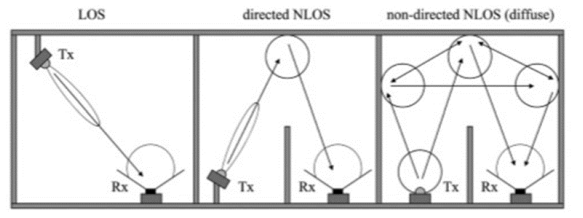
\includegraphics[width=0.75\textwidth,keepaspectratio]
			{channel.png}
		\end{center}
		\caption{Mô hình kênh truyền trong hệ thống VLC } 
		
	\end{figure}
\end{center}		

\subsubsection{Suy hao (Pathloss)}

Kênh truyền đơn giản nhất là kênh truyền không gian tự do \ac{los}, trong mô hình này ta không
xét đến bất kỳ vật thể nào ở giữa hai phía phát và thu. Trong trường hợp đơn giản này, tín hiệu phát bị suy hao do
năng lượng trải đều xung quanh an ten phát. Đối với mô hình này, công suất nhận được là:

\begin{equation}
	P_T=P_t[\dfrac{\sqrt{G_L} \lambda}{4 \pi d}]^2
	\label{reg:suyhao}
\end{equation}


Trong đó, $P_t$ là công suất phát, $G_L$ là tích biểu đồ bức xạ trường của anten phát và thu, $\lambda$ là bước sóng và d
là khoảng cách giữa hai phía. Theo lý thuyết, công suất suy giảm tỉ lệ với bình phương khoảng cách, nhưng trong
thực tế, công suất suy giảm rất nhanh, thông thường là lũy thừa bậc 3 hoặc 4 so với khoảng cách. Sự tồn tại của
mặt đất ở trên kênh truyền, đóng vai trò là mặt phản xạ của các sóng tới. Những sóng phản xạ này thường ngược
pha so với sóng tới, và có thể làm giảm công suất nhận được. Xét thêm sự ảnh hưởng của mặt đất, suy hao kênh
truyền có thể được tính như sau:

\begin{equation}
	P_T=P_t \dfrac{G_t G_T h_t^2 h_r^2}{d^4}
\end{equation}

Ở đây, $h_t$ và $h_r$ là chiều cao của anten phát và anten thu. Công thức trên khác với \eqref{reg:suyhao}  ở một số
điểm sau, có sự ảnh hưởng của chiều cao anten, không xét đến bước sóng, và ảnh hưởng của khoảng cách d là lũy
thừa bậc 4. Thông thường, công thức mang tính thực tiễn kinh nghiệm cao hơn, được sử dụng để tính toán suy hao
kênh truyền là:

\begin{equation}
	P_T=P_t P_0 [\dfrac{d_0}{d}]^\alpha
\end{equation}
	
	Trong đó, $P_0$ là công suất tại vị trí mẫu $d_0$, và $\alpha$ là hệ số suy hao kênh truyền. Từ công thức trên, suy hao
	kênh truyền theo mô hình logarit được tính như sau:
	
	\begin{equation}
		PL(d)dB=\hat{PL}(d_0)+10 \alpha log(\dfrac{d}{d_0})
	\end{equation}
Trong đó, $\hat{PL}(d_0)$ là suy hao trung bình theo dB tại khoảng cách $d_0$.

\subsubsection{Shadowing}

Nếu có sự tồn tại của các vật thể (tòa nhà, cây cối,...) dọc đường đi của tín hiệu, một vài phần của tín hiệu
phát đi có thể mất mát do sự hấp thụ, phản xạ, tán xạ, nhiễu xạ. Những ảnh hưởng này còn gọi là shadowing. Như \ref{fig:shadowing}
được mô tả trong , vật thể ở giữa đã chắn đường đi của tín hiệu từ phía phát đến phía thu.

\begin{center}	
	\begin{figure} [ht]
		\begin{center}
			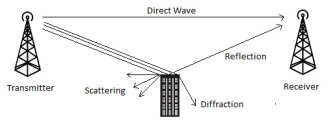
\includegraphics[width=0.75\textwidth,keepaspectratio]
			{shadowing.png}
		\end{center}
		\caption{Mô hình kênh truyền chịu sự ảnh hưởng của shadowing } 
		\label{fig:shadowing}
	\end{figure}
\end{center}

Suy hao kênh truyền shadowing:

\begin{equation}
	PL(d)dB=\hat{PL}(d_0)+10 \alpha log(\dfrac{d}{d_0}) + \chi
\end{equation}

Ở đây, $\chi$ là biến phân bố ngẫu nhiên chuẩn hóa với độ lệch chuẩn $\sigma$, $\chi$ đại diện cho sự ảnh hưởng của
shadowing. Do kết quả của hiện tượng này, nên công suất thu được tại những điểm có cùng khoảng cách đến anten
phát có thể khác nhau, và có phân bố logarit chuẩn hóa.

\subsubsection{Hiện tượng đa đưởng (multipath)}

Những vật thể nằm trên đường đi của tín hiệu sẽ đóng vai trò là mặt phản xạ tín hiệu, một số các tín hiệu
phản xạ cũng được nhận tại phía thu. Bởi vì mỗi tín hiệu này đi trên những con đường khác nhau, chúng sẽ có biên
độ và pha khác nhau như \ref{fig:multipath}.

\begin{center}	
	\begin{figure} [ht]
		\begin{center}
			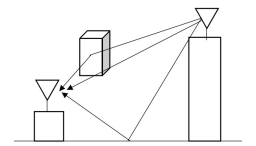
\includegraphics[width=0.75\textwidth,keepaspectratio]
			{multipath.png}
		\end{center}
		\caption{Mô hình kênh truyền chịu sự ảnh hưởng của multipath } 
		\label{fig:multipath}
	\end{figure}
\end{center}

Phụ thuộc vào pha của chúng khi tới được phía phát, những tín hiệu này có thể làm giảm hoặc tăng công
suất thu được. Chỉ một thay đổi nhỏ về vị trí cũng có thể khiến cho biên độ và pha của tín hiệu tới vô cùng khác
nhau. Ba thành phần của đáp ứng kênh truyền được mô tả khá rõ trong \ref{fig:tong}.

\begin{center}	
	\begin{figure} [ht]
		\begin{center}
			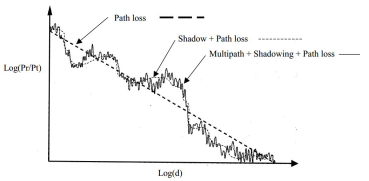
\includegraphics[width=0.75\textwidth,keepaspectratio]
			{tong.png}
		\end{center}
		\caption{Suy hao, shadowing và hiệu ứng đa đường } 
		\label{fig:tong}
	\end{figure}
\end{center}






	
\subsubsection{Các tham số hiệu năng của kênh truyền}

\textbf{a) Tỉ số tín hiệu trên nhiễu SNR (Signal-to-Noise Ratio)}

Hàm mật độ công suất nhiễu có thể được xác định như sau:

\begin{equation}
	N_{0}\cong N_{Shot}=2qyP_{n}\sim10^{-22}(\dfrac{A^2}{Hz})
\end{equation}

Trong đó:

y là hệ số đáp ứng

$P_{n}$ là năng lượng ánh sáng trung bình

Từ đó, với mỗi tốc độ bit $R_{b}$ nào đó và $P_{r}$ là công suất quang nhận được, ta có tỉ lệ lỗi bit SNR được xác định như sau:

\begin{equation}
	SNR=\dfrac{y^2P_{r}^2}{R_{b}N{0}}
\end{equation}
\vspace{\baselineskip}
\textbf{b) Dung năng kênh}

Theo định lý Shannon, dung năng kênh C ( tốc độ truyền dữ liệu tối đa ứng với một giá trị SNR cho trước) được xác định bởi:

\begin{equation}
	C=Blog_2(1+SNR)
\end{equation}

\textbf{c) Tỉ lệ lỗi bit BER (Bit Error Rate)}



\begin{equation}
	BER=\dfrac{Error bits}{bits}
\end{equation}

Mức ngưỡng BER của hệ thống là 0.0038.

\vspace{\baselineskip}
Những kiến thức trên là từ hệ thống thông tin vô tuyến nói chung, do đó hệ thống VLC có đôi chút khác
biệt. Do hệ thống VLC sử dụng chủ yếu ở môi trường trong nhà, kênh truyền ít biến động, nên trong bản báo cáo
này ta xét mô hình LOS cho hệ thống. \eqref{eq:los} mô tả suy hao kênh truyền trong kịch bản LOS-VLC
(Line of sight visible light communication). Trong công thức đó, khoảng cách giữa bên thu với bên phát là D và độ
mở của bộ thu là r. Góc hợp bởi đường thẳng nối giữa phía phát và phía thu với trục máy thu là $\alpha$ và với trục máy
phát là $\beta$. $\omega_r$ là góc quan sát của máy thu, và $A_r$ là diện tích thu.

\begin{equation}
	A_rcos(\alpha)=D^2 \omega_r
	\label{eq:los}
\end{equation}

\begin{center}	
	\begin{figure} [ht]
		\begin{center}
			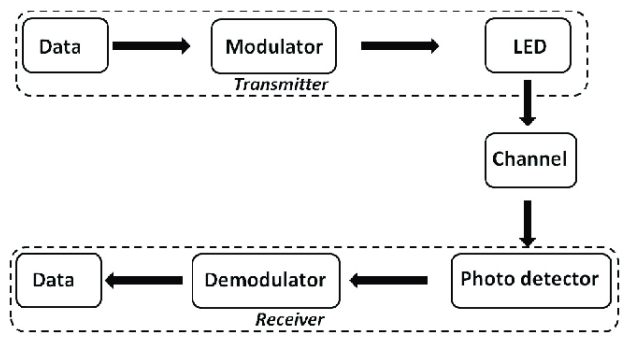
\includegraphics[width=0.75\textwidth,keepaspectratio]
			{hethongvlc.png}
		\end{center}
		\caption{Kênh truyền hệ thống VLC } 
		
	\end{figure}
\end{center}	

Do đây là hệ thống VLC, nên yếu tố ánh sáng cũng phải được xem xét. Luồng ánh sáng hấp thu được ở phía
thu và suy hao kênh truyền ánh sáng lần lượt được tính theo \eqref{reg:thu}

\begin{equation} 
	F_r=log_s(\beta) \omega_r
	\label{reg:thu}
\end{equation}

\begin{equation} 
	L_L=\dfrac{F_r}{F_s}=\dfrac{g_s(\beta)A_rcos(\alpha)}{D^2\int_{0}^{\Theta_max}2\pi g_s(\Theta)sin(\theta)d\theta}
	\label{reg:mat}
\end{equation}

Trong những phương trình trên, $g_s(\beta)$ là hàm phân bố ánh sáng chuẩn hoá, được cung cấp bởi nhà phân phối thiết bị. Đơn giản hoá \eqref{reg:mat}, suy hao kênh truyền LOS được tính toán với bậc lambert $m=\dfrac{\ln(2)}{ln(cos(\alpha 1/2)}$ và góc nửa công suất của phía thu $\alpha_(1/2)$. Trong \eqref{reg:mat}, $\beta$ đại diện cho góc \ac{fov} của máy thu, $A_r$ là diện tích hấp thụ của bộ thu. DO đó , hệ số kênh truyền phụ thuộc vào vị trí của máy thu so với máy phát. Như vậy, suy hao kênh truyền tổng quát của hệ thống VLC được tính theo công thức 

\begin{equation}
	L_L=\dfrac{(m+1)A_r}{2\pi D^2}cos(\alpha)cos^m(\beta)
\end{equation}

\begin{center}	
	\begin{figure} [ht]
		\begin{center}
			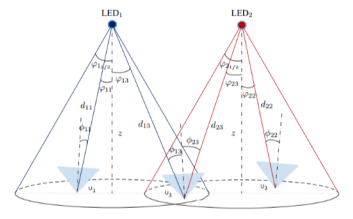
\includegraphics[width=0.75\textwidth,keepaspectratio]
			{loslos.png}
		\end{center}
		\caption{Mô hình MIMO trong phòng } 
		
	\end{figure}
\end{center}	



\subsubsection{Hệ thống MIMO quang không dây}
Cách tiếp cận dựa trên việc sử dụng kỹ thuật \ac{mimo},
liên quan đến truyền thông không dây, có nghĩa là dữ liệu
được truyền dưới dạng nhiều hơn một luồng, như vậy
cách mà nhiều con đường truyền được tạo thành
đồng thời, giữa nhiều anten phát
và nhiều anten thu. Tất nhiên, khi
chúng ta nói về việc thực hiện truyền MIMO trong
lĩnh vực quang học, chúng ta đang suy nghĩ về nhiều
bộ phát và dò ánh sáng thay vì ăng-ten vô tuyến.
Tuy nhiên, ý tưởng chính vẫn được duy trì. Nếu chúng ta
nói về hệ thống VLC trong nhà, nơi có đèn LED
 được sử dụng làm nguồn sáng, thường được cấu thành từ
nhiều đèn LED riêng biệt. Về mặt lý thuyết, có thể tách các bộ truyền dữ liệu riêng lẻ ở cả mức độ
toàn bộ bóng đèn, nếu nhiều hơn một bóng đèn được lắp đặt trong cùng một nơi, cũng như số lượng của đèn LED riêng lẻ hoặc
các nhóm bên trong một bóng đèn. Bất kể trường hợp nào trong thực tế,  sự hoạt động của
hệ thống MIMO-VLC có thể được mô tả bằng một mô hình toán học, giải thích bằng đồ thị được mô tả ở \ref{fig:MIMOsys}. Trong hệ thống truyền dẫn như vậy, các tín hiệu được truyền đồng thời bởi N máy phát và M máy thu, trong đó ($M>=N$) được mô tả bởi phương trình sau \cite{2x2}:

\begin{equation}
	X=HY+n
\end{equation}

Trong đó X là vectơ của tín hiệu truyền, Y là vectơ tín hiệu nhận, H là ma trận của kênh truyền chuẩn.

\vspace{\baselineskip}
Ma trận này được hình thành bởi độ truyền giữa
mỗi máy phát và mỗi máy thu, và có thể được ước tính
bằng độ lợi giữa máy thu thứ i và máy phát thứ j. Bằng cách nghịch đảo ma trận H, ta có thể phục hồi lại tín hiệu ban đầu, theo công thức:

\begin{equation}
	Y=H^{-1}X+n
\end{equation}
 
Hiển nhiên,ma trận H có thể không phải là ma trận 1 chiều và điều kiện của nó quyết định \ac{snr}. Ma trận $H^{-1}$ có thể được tìm thấy bởi 1 số thuật toán tối ưu hoá hoặc được tính toán ở giai đoạn khởi tạo hệ thống. Trong thực tế, phương pháp cuối cùng là thường được sử dụng. Bởi vì quá trình phục hồi tín hiệu ở bên thu , kiến thức về ma trận $H^{-1}$ là cần thiết, hệ thống hoạt động tốt hơn ở 2 pha. Ở pha đầu tiên, ma trận H được định nghĩa, thông thường 1 số tín hiệu pilot được truyền. Dựa vào đó, ma trận $H^{-1}$ được tính.Ở giai đoạn 2, tín hiệu chứa thông tin được truyền. Ma trận $H^{-1}$ được sử dụng trong quá trình khôi phục tín hiệu. 
\begin{center}	
	\begin{figure} [ht]
		\begin{center}
			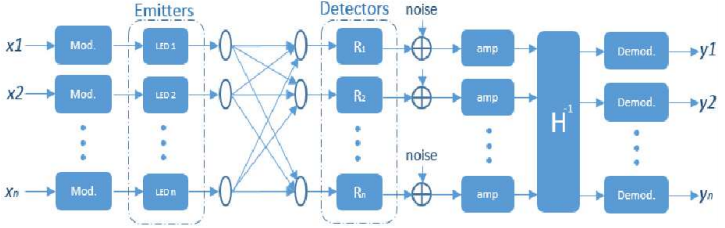
\includegraphics[width=0.85\textwidth,keepaspectratio]
			{mimoxanh.png}
		\end{center}
		\caption{Mô hình của hệ thống giao tiếp ánh sáng MIMO } 
		\label{fig:MIMOsys}
	\end{figure}
\end{center}





	
\section{Neural Network}
	
	\subsection{Mạng thần kinh học}
	Bộ não con người là một hệ thống xử lý thông tin phức hợp, phi tuyến và song song có khả năng học, ghi nhớ, tổng quát hóa và xử lý lỗi. Những khả năng có được của não bộ là nhờ nó được cấu thành từ một mạng thần kinh chứa rất nhiều tế bào neural sinh học và con số đó được ước tính khoảng 100 tỷ tế bào.
	
\begin{center}	
	\begin{figure} [ht]
		\begin{center}
			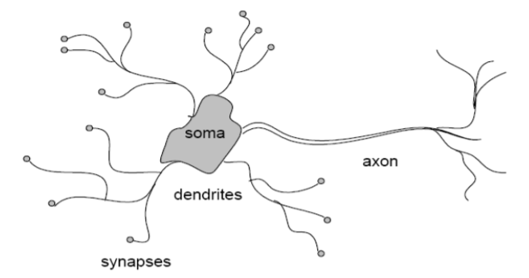
\includegraphics[width=0.75\textwidth,keepaspectratio]
			{mangnoron.png}
		\end{center}
		\caption{Sơ đồ 1 neural sinh học  } 
		
	\end{figure}
\end{center}	

Mỗi neural nhận xung thần kinh (thông tin) truyền từ neural đứng trước nó, truyền dọc theo Axon và truyền ra neural sau thông qua Synapse. Xung động thần kinh truyền từ neural này sang neural khác trong mạng thần kinh tạo nên mọi chức năng thần kinh của não bộ.

\vspace{\baselineskip}
Con người với ước muốn nhân tạo hóa mạng thần kinh sinh học nên đã tìm cách mô phỏng cách não bộ hoạt động bằng máy tính và các thuật toán để phục vụ nhiều mục đích trong đời sống.

\subsection{Mạng thần kinh nhân tạo}
Mạng thần kinh nhân tạo (Artificial neural network – ANN) là mô hình xử lý thông tin được mô phỏng dựa trên hoạt động của hệ thống thần kinh sinh vật, bao gồm số lượng lớn các neural được gắn kết thông qua các trọng số liên kết để xử lý thông tin. ANN giống như não bộ con người, được học bởi kinh nghiệm (thông qua huấn luyện), có khả năng lưu giữ những kinh nghiệm hiểu biết (tri thức) và sử dụng những tri thức đó trong việc dự đoán những dữ liệu chưa biết.
 
\vspace{\baselineskip}
Người ta phân loại mạng neural dựa vào các kiểu kết nối của các neural và dựa vào số lớp neural trong mạng:

\begin{itemize}
	\item Phân loại dựa theo kiểu kết nối các neural: dựa theo kiểu kết nối, ta có mạng neural truyền thẳng (feedfoward Neural Network) và mạng hồi quy (recurrent NN). Trong mạng truyền thẳng, các kết nối đi theo một hướng nhất định, không tạo thành chu trình. Ngược lại, các mạng hồi quy cho chép các kết nối neural tạo thành chu trình, với đỉnh là các neural và cung là các kết nối giữa chúng. Các neural nhận tín hiệu vào gọi là neural vào, các neural đưa thông tin ra gọi là neural ra, các neural còn lại gọi là neural ẩn.
	\item Phân loại theo số lớp neural: các neural trong mạng có thể được tổ chức thành các lớp theo nguyên tắc neural ở lớp này, chỉ được nối với các neural ở lớp khác, không cho phép kết nối giữa các neural trên cùng một lớp, hoặc từ neural lớp dưới lên neural lớp trên. Lớp nhận tín hiệu vào gọi là lớp vào, lớp đưa thông tin ra gọi là lớp ra, các lớp ở giữa gọi là lớp ẩn. Thông thường lớp vào không tham gia quá trình tính toán của mạng neural, nên khi tính số lớp người ta không kể lớp vào.
\end{itemize}

\subsubsection{Kiến thức cơ bản của mạng thần kinh nhân tạo}
Perceptron: Tên gọi của các neuron trong mạng thần kinh nhân tạo(ANN). Nó có chức năng nhận đầu vào và xuất đầu ra.

\begin{center}	
	\begin{figure} [ht]
		\begin{center}
			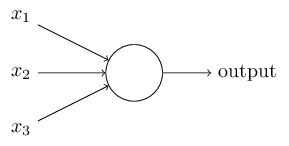
\includegraphics[width=0.5\textwidth,keepaspectratio]
			{perceptron.png}
		\end{center}
		\caption{Cấu trúc của 1 perceptron } 
		
	\end{figure}
\end{center}	

Một ANN cấu thành từ nhiều lớp khác nhau, trong đó gồm:

\begin{itemize}
	\item Lớp vào (Input layer): có chức năng nhận dữ liệu đầu vào.
	\item Lớp ẩn (Hidden layer): nhận dữ liệu từ các lớp trước nó, sau đó xử lý và lan truyền dữ liệu đến các lớp tiếp theo. Trong một ANN thường có nhiều lớp ẩn, số lượng sẽ phụ thuộc vào người thiết kế mạng.
	\item Lớp ra (Output layer): tổng hợp thông tin nhận được và cho ra kết quả tính toán của mạng.
\end{itemize}

\begin{center}	
	\begin{figure} [ht]
		\begin{center}
			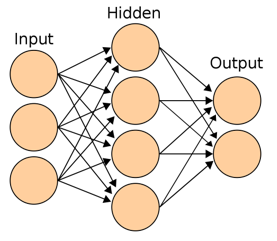
\includegraphics[width=0.5\textwidth,keepaspectratio]
			{ANN.png}
		\end{center}
		\caption{Cấu trúc của 1 mạng ANN } 
		
	\end{figure}
\end{center}	

\subsection{Probabilistic neural network (PNN)}
\subsubsection{Kiến thức cơ bản về PNN}
Mạng nơ-ron xác suất \ac{pnn} là một mạng nơ-ron truyền thẳng (các kết nối giữa các nơ-ron không tạo thành 1 chu trình), được xử dụng nhiều trong các bài toán phân lớp và nhận diện đặc điểm. Trong thuật toán PNN, hàm mật độ xác suất mẹ  \ac{pdf} của từng lớp đươc tính gần bằng bằng cửa  sổ parzen và một hàm phi tham số. \ac{pdf}  của mỗi lớp sau đó được sử dụng để tính xác suất lớp của dữ liệu đầu vào mới cùng với quy tắc Bayes được áp dụng để phân bổ lớp có xác suất cao nhất cho lớp dữ liệu đầu vào mới. Loại \ac{ann} này được bắt nguồn từ mạng Bayes  và một thuật toán thống kê được gọi là phân tích phân biệt Kernel Fisher, được giới thiệu bởi D.F. Specht năm 1966 \cite{pnn}.

	\begin{center}	
	\begin{figure} [ht]
		\begin{center}
			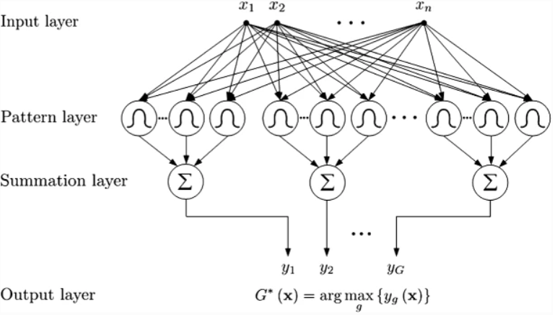
\includegraphics[width=0.75\textwidth,keepaspectratio]
			{PNN.png}
		\end{center}
		\caption{Sơ đồ cấu trúc một PNN} 
	\end{figure}
\end{center}
 
PNN có 4 lớp như sau: Input layer (Lớp đầu vào), Pattern layer (Lớp mẫu), Summation layer (Lớp tổng hợp), Output layer (Lớp đầu ra).

\vspace{\baselineskip}
a)	Input layer (Lớp đầu vào):

Mỗi neural trong lớp này đại diện cho một biến cần dự đoán x1, x2, …, xn, nó nhận giá trị của biến dự đoán sau đó cung cấp cho từng neural trong lớp ẩn.

\vspace{\baselineskip}
b)	Pattern layer (Lớp mẫu):

Số neural trong lớp này ứng với số trường hợp trong tập dữ liệu huấn luyện – các vector đặc trưng và nhãn của nó (giả sử có G nhãn trong PNN).
 
\vspace{\baselineskip}
Mỗi nút trong lớp này chứa tương ứng với một hàm Gauss cho mỗi vector đặc trưng mẫu. Hàm Gauss này tập trung vào vector đặc trưng liên kết của nó.

\vspace{\baselineskip}
Đầu ra của mỗi nút được tính theo công thức sau:

\begin{equation}
	f_i=\dfrac{1}{\sqrt{(2\pi\sigma_g^2)^N}}e^{-\dfrac{\parallel x_i-x^{(p)} \parallel ^2}{2\sigma_g^2}}
\end{equation}

Trong đó: 

\begin{itemize}
	\item $\sigma_g$ : là độ lệch chuẩn của hàm gauss ứng với mỗi nhãn nó có thể bằng một nửa khoảng cách từ mẫu đến vector mẫu khác gần nhất.
	
	\item $x_i$ : là vector đầu vào cần xác định nhãn.
	
	\item N	: là kích thước vector mẫu đầu vào $x_i$
	
	\item p	: là số lượng mẫu đặc trưng cho một nhãn
	
	\item $\parallel x_i-x_{(p)} \parallel$ : là khoảng cách Euclide (căn bậc hai của tổng bình phương) giữa $x_i$ và $x_{(p)}$
	
\end{itemize}

\vspace{\baselineskip}
c)	Summation layer (Lớp tổng hợp): 

Ta có G neural trong lớp này ứng với số lượng nhãn trong mạng, mỗi nút cung cấp giá trị cho lớp đầu ra $y_g$,  bằng cách tính tổng các giá trị đầu vào nhận được từ các neural lớp mẫu của từng nhãn tương ứng. Các giá trị $y_g$ này ta gọi là trọng số của phiếu bầu cho nhãn mục tiêu ứng với $x_i$.

\vspace{\baselineskip}
d)	Output layer (Lớp đầu ra): 

Nhiệm vụ lớp này so sánh các phiếu bầu có trọng số được nhận từ lớp tổng hợp, nhãn có trọng số phiếu bầu lớn nhất được dùng để dự đoán loại mục tiêu cho đầu vào $x_i$.

\subsubsection{Cửa sổ Parzen}

1 trong những thuật toán phi tham số để ước tính \ac{pdf} là "cửa sổ Parzen". Để tính toán \ac{pdf} $p(x)$ tại điểm x, yêu cầu xác định số mẫu $N_h$ với khoảng $[x-h,x+h]$ và chia cho tổng số vectơ mẫu M và 2h. Công thức ước lượng \ac{pdf} tại x

\begin{equation}
	\hat{p}(x)=\dfrac{N_h(x)}{2hM}
	\label{eq:dat}
\end{equation}

Với hàm hỗ trợ $k_h$, ta có thể chọn


	$$
	K_h=
	\begin{cases}
		0,5 & \text{nếu} |m|<=|1|\\
	0 & \text{nếu} |m|>|1|
	\end{cases}
$$




Từ \eqref{eq:dat} chúng ta có

\begin{equation}
	\hat{p}(x)=\dfrac{1}{hM} \sum_{i=1}^{M} K(\dfrac{x-m}{h})
\end{equation}

Với tổng thứ i bằng không khi $m_i$ không thuộc khoảng $[x-h,x+h]$, điều này dẫn đến

\begin{equation}
	\gamma (x,m) = \dfrac{1}{h} K(\dfrac{x-m}{h})
\end{equation}

Nếu như $\hat{p}$ được xem như hàm liên quan đến số lượng mẫu, chúng ta suy ra

\begin{equation}
	\hat{p}(x)=\hat{p}(x,M)
\end{equation}

$\hat{p}$  không sai lệch khi $M \rightarrow \infty$, nếu $h=h(M)$

Trong thực tế, chỉ xảy ra với những số hữu hạn. Lựa chọn cho thông số h là cực kì quan trọng, vì thế được khuyến khích bắt đầu từ ước lượng ban đầu của h rồi sau đó thay đổi từ từ để giảm thiểu sai số phân lớp sai. 1 cách lý thuyết, số M lớn là cần thiết. Nhưng trong thực tế, 1 số lượng lớn các điểm làm tăng sự phức tạp tính toán 1 cách không cần thiết.

\vspace{\baselineskip}
Sự lựa chọn thông thường của hàm $K(m)$ là

\begin{equation}
	K(m)=(2\pi)^{1/2}e^{\dfrac{-m^2}{2}}
\end{equation}

\begin{equation}
	K(m)=\dfrac{1}{\pi (1+m^2)}
\end{equation}

$$
K(m)=
\begin{cases}
	1-|m| & \text{nếu} |m|<=|1|\\
	0 & \text{nếu} |m|>|1|
\end{cases}
$$

\subsubsection{Thuật toán Bayes cho bài toán phân lớp}
1 quy chuẩn được chấp nhận cho các quy tắc lựa chọn hoặc chiến lược được dùng để giải bài toán phân lớp là chúng làm theo cách mà giảm thiểu "rủi ro mong đợi".Chiến lược như vậy gọi là "chiến lược Bayes và có thể được ứng dụng trong các vấn đề chứa nhiều thể loại.
 
\vspace{\baselineskip}
Xem xét 1 tình huống 2 loại trong đó trang thái của $\theta$ được biết là $\theta_A$ hoặc $\theta_B$. Nếu như bài toán mong muốn xác định $\theta = \theta_A$ hoặc $\theta = \theta_B$ dựa trên 1 tập các chỉ số đo được biểu hiện bởi 1 vector có $\rho$ chiều $X^t = [X_1..X_2..X_3]$,quy tắc Bayes trở thành \cite{bay}

\begin{align}
	\begin{split}
		d(X) = \theta_A , & \text{nếu $h_A I_A f_A (X) > h_B I_B f_B (X)$} \\
		d(X) = \theta_B , & \text{nếu $h_A I_A f_A (X) < h_B I_B f_B (X)$}
	\end{split}
\end{align}

Trong đó $f_A (X)$ và $f_B (X)$ là các hàm mật độ xác suất \ac{pdf} cho loại A và loại B. $I_A$ là hàm mất mát với quyết định $d(X) = \theta_B$ khi $\theta = \theta_A$; $I_B$ là hàm mất mát với quyết định $d(X)= \theta_A$ khi $\theta = \theta_B$ (Sự mất mát liên quan đến quyết định đúng sẽ bằng 0). $h_A$ là xác suất giả thuyết của dữ liệu quan sát thuộc loại A và $h_B=1-h_A$ là xác suất giả thiết khi $\theta = \theta_B$.

\vspace{\baselineskip}
Do đó đường biên giới giữa các vùng trong đó quyết định Bayes $d(X) = \theta_A$ và vùng trong đó $d(X) = \theta_B$ được chi bởi 

\begin{equation}
	f_A(X) = Kf_B(X)
	\label{eq:aa}
\end{equation}

Trong đó

\begin{equation}
	K=h_BI_B / h_AI_A
\end{equation}

Thông thường, 2 loại quyết định được cho bởi \eqref{eq:aa} có thể phức tập tuỳ ý, khi không có 1 giới hạn cho mật độ ngoại trừ các điều kiện mà hàm mật độ xác suất phải tuân theo, ví dụ như chúng có thể không âm, tích hợp và các tích phân của chúng trong mọi không gian đều bằng nhau. Các quy luật quyết định tương tự có thể được dùng trong mọi bài toán nhiều loại.

\vspace{\baselineskip}
Chìa khoá để sử dụng \eqref{eq:aa} là khả năng dự đoán \ac{pdf} dựa trên các tập training. Thông thường xác suất giả thuyết có thể được biết hay được dự đoán chính xác và hàm mất mát yêu cầu sự đánh giá chủ quan. Tuy nhiên, nếu mật độ xác suất của mẫu thuộc loại bị phân chia là không biết, và tất cả được cho bởi 1 tập training mẫu, khi đó mẫu này chỉ cung cấp bằng chứng cho mật độ xác suất quan trọng chưa biết.
	
	


\subsubsection{Ưu điểm và nhược điểm của PNN}
Mạng nơ-ron xác suất có nhiều ưu và nhược điểm so với mạng nơ-ron nhiều lớp truyền thống

\vspace{\baselineskip}
\textbf{a) Ưu điểm:}

\begin{itemize}
	\item \ac{pnn} nhanh hơn sơ với mạng nơ-ron nhiều lớp truyền thống.
	\item \ac{pnn} cho kết quả chính xác hơn so với mạng nơ-ron nhiều lớp truyền thống.
	\item \ac{pnn} tương đối nhạy cảm với những ngoại lệ.
	\item \ac{pnn} tạo ra các điểm xác suất mục tiêu dự đoán chính xác.
	\item \ac{pnn} tiệm cận phân loại tối ưu Bayes.
\end{itemize}

\textbf{b) Khuyết điểm:}

\begin{itemize}
	\item \ac{pnn} chậm hơn mạng nơ-ron nhiều lớp truyền thống ở phân loại các trường hợp mới.
	\item \ac{pnn} yêu cầu nhiều bộ nhớ để lưu trữ mô hình
\end{itemize}

\subsubsection{Cách ứng dụng mạng nơ-ron xác suất vào đề tài luận văn}

Trong đề tài luận văn này, tín hiệu được sử dụng là tín hiệu NRZ 2 mức 0 và 1,sau khi đi qua hệ thống sẽ bị biến đổi thành tín hiệu có các mức khác nhau. Bài toán đặt ra ở bộ cân bằng là làm thế nào để biến đổi các mức tín hiệu khác nhau về thành tín hiệu ban đầu có 2 mức 0 và 1. Bài toán này tương tự như bài toán phân lớp nên chúng em quyết định chọn mạng nơ-ron xác suất đề giải quyết vấn đề. Ngoài ra còn 1 điểm nữa là mô hình \ac{pnn} là 1 hàm có sẵn trong matlab mà còn rất tối ưu nên rất thuận tiện cho việc xử lý chuỗi tín hiệu lên đến hàng ngàn bit.

\begin{center}	
	\begin{figure} [ht]
		\begin{center}
			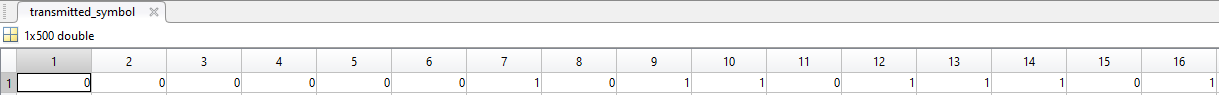
\includegraphics[width=1\textwidth,keepaspectratio]
			{transbit.png}
		\end{center}
		\caption{1 chuỗi gồm 500 bit ngẫu nhiên 0 và 1 được tạo từ code Matlab } 
		
	\end{figure}
\end{center}	

\begin{center}	
	\begin{figure} [ht]
		\begin{center}
			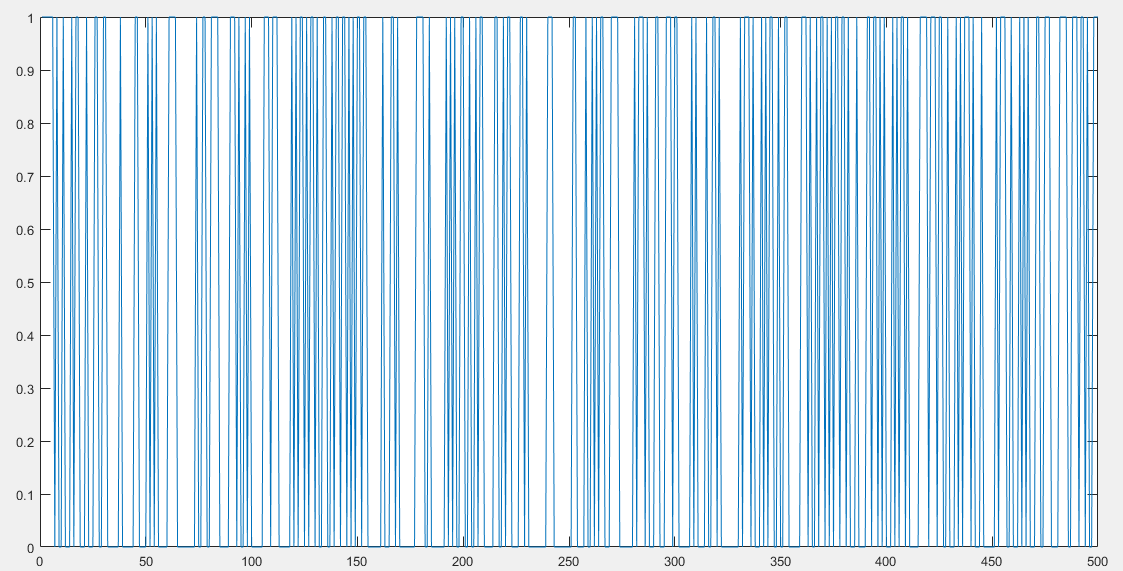
\includegraphics[width=0.75\textwidth,keepaspectratio]
			{signalbits.png}
		\end{center}
		\caption{Hình ảnh của chuỗi được đưa vào máy phát sóng } 
		
	\end{figure}
\end{center}	

Sau khi đi qua hệ thống thực tế, tín hiệu sẽ bị suy hao + méo dạng như hình \ref{fig:thu}.Khi phân tích, ta sẽ nhận được 1 chuỗi gồm 500 symbols nhưng mỗi symbols sẽ được biễu diễn bởi các 3 mức khác nhau như hình \ref{fig:sig}. Bằng cách xử dụng \ac{pnn} , ta sẽ biển đỗi 3 samples đấy về thành 1 mức 0 hoặc 1 cho giống với chuỗi truyền đi. Như vậy đây là bài toán phân lớp 1500 điểm về thành 2 lớp 0 hoặc 1.

\begin{center}	
	\begin{figure} [ht]
		\begin{center}
			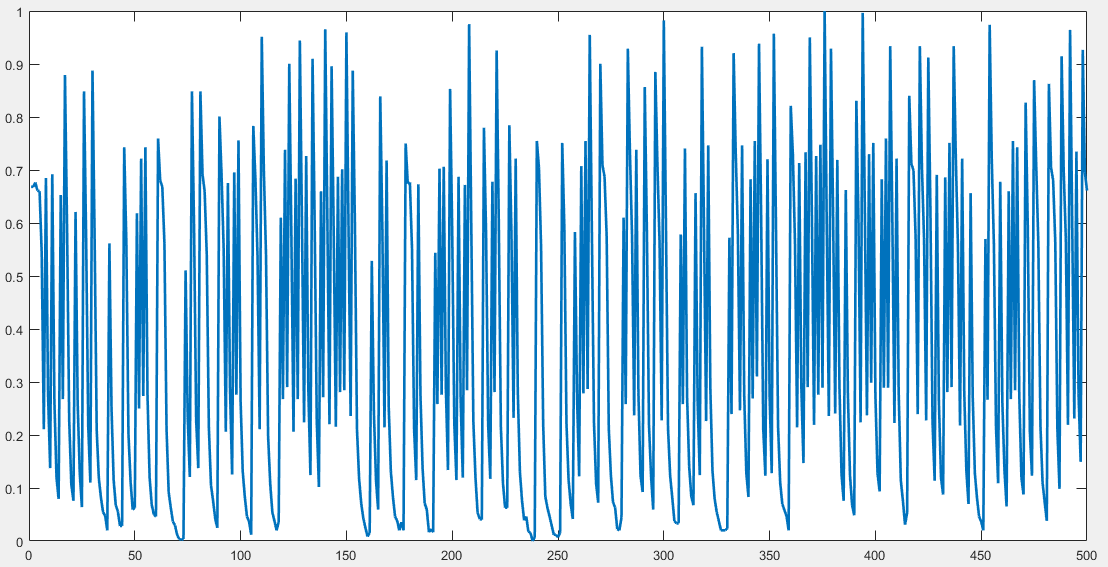
\includegraphics[width=0.75\textwidth,keepaspectratio]
			{SRbits.png}
		\end{center}
		\caption{Hình ảnh của chuỗi bit thu được  } 
		\label{fig:thu}
		
	\end{figure}
\end{center}	

\begin{center}	
	\begin{figure} [ht]
		\begin{center}
			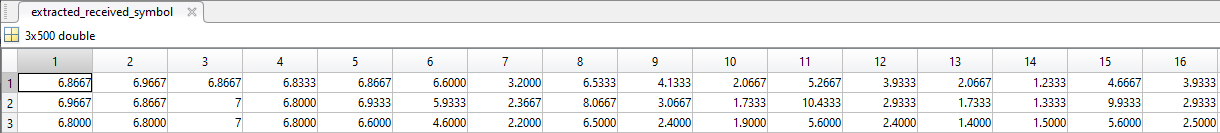
\includegraphics[width=1\textwidth,keepaspectratio]
			{Rbits.png}
		\end{center}
		\caption{Chuỗi bit thu được gồm 500 symbols và 1 symbols được biễu diễn bởi 3 samples  } 
		\label{fig:sig}
		
	\end{figure}
\end{center}

\section{Kết luận chương}

Trong đề tài, tín hiệu NRZ được sử dụng 2 mức 0 và 1 được sử dụng vì ít tiêu tốn băng thông với lại đơn giản, dễ dàng quan sát khi có lỗi xuất hiện khi chuỗi tín hiệu phát đi là 1 chuỗi dài.

\vspace{\baselineskip}
Tín hiệu thu được từ hệ thống thực tế sẽ bị nhiễu phi tuyến + đường truyền không ổn định vì thế phương pháp mạng nơ-ron nhân tạo được sử dụng với các lý do kể trên.
 
\vspace{\baselineskip}
Ở chương kết tiếp ,các thông số cụ thể của hệ thống MIMO-VLC cũng như các bước thực hiện thí nghiệm, kết quả và đánh giá phương pháp neural network sẽ được trình bày.







\chapter{KẾT QUẢ NGHIÊN CỨU} \label{sec:chapter_3}
\section{Phương pháp tiếp cận}
\subsection{Hệ thống VLC}
\begin{figure} [H]
	\centering
	\captionsetup{justification=centering}
	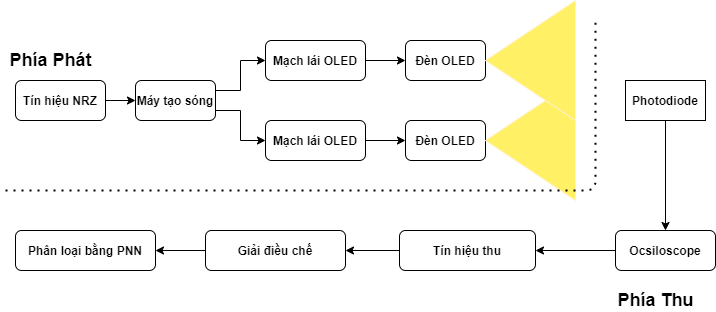
\includegraphics [scale=0.5]
	{ThuPhat.png}
	\caption{Hệ thống \ac{vlc} thực tế tại phòng thí nghiệm 209B1}
\end{figure}
\begin{table}[H]
	\caption{Bảng các thành phần của hệ thống VLC thực tế}.
	\begin{center}
		\small
		\begin{tabular}{|c|c|}
			\hline
			Thiết bị & Thông số\\
			\hline
			\multirow{2}{*}{Generator AFG 3152C}
			&Tốc độ lấy mẫu tối đa 1GS/s, 2 kênh, băng thông 150MHz\\
			&Có thể phát dạng sóng Sine, Square, Pulse, Ramp, Guassian,…. \\			
			&Điều chế AM, FM, PM, FSK, PWM \\
			&Nguồn 100 - 240 V, 47 - 63 Hz\\
			\hline
			\multirow{2}{*}{Oscilloscope}
			&Tốc độ lấy mẫu tối đa 1GS/s\\
			&Băng thông 50MHz\\ 
			&Void/Div tối thiểu 2mV\\
			\hline
			\ac{oled} & Băng thông khoảng 4.3kHz\\
			\hline
			\multirow{2}{*}{Photodiode (PD)}
			& PDA36A của ThorLab \\
			& Bước sóng từ 350 – 1100 nm \\
			& Độ lợi tùy chỉnh từ 0 đến 70 dB \\
			& Điện áp tối đa 5 V và trở kháng 50 $\Omega$ \\
			\hline
			\multirow{2}{*}{Nguồn DC}
			& Điện áp 1.1 - 1.3 V \\
			& Cường độ dòng điện 0.7 - 0.9 A \\
			\hline
		\end{tabular}
		\label{tab:VLC_info}
	\end{center}
\end{table}
\newpage
\subsection{Dữ liệu}
Dữ liệu được sử dụng trong bài toán này là tín hiệu \ac{nrz} thu được từ photodiode. Tín hiệu thu được trong khoảng tần số từ 40kHz đến 63kHz, khoảng cách từ 25 cm đến 150 cm. Mỗi chuỗi thu được từ Ocsiloscope
bao gồm 2500 điểm.

Để đánh giá tín hiệu thu được một cách tổng quát, chúng ta dùng thông số là BER được tính dựa trên SNR. SNR được tính dựa trên giản đồ mắt, có giá trị bằng:
\begin{equation}
	SNR  = \frac{mean(highlevel) - mean (lowlevel)}{\sigma(highlevel) + \sigma(lowlevel)}
\end{equation}
Công thức trên được tính theo V, nên cần đổi ra dB bằng cách lấy $20\log_{10}$ kết quả ở trên.

\ac{ber} được tính theo công thức sau:
\begin{equation}
	BER = \frac{1}{2} erfc (\sqrt{SNR})
\end{equation}
Đây chính là số bit lỗi được ước lượng dưa trên tín hiệu thu được mà chưa qua mạng nơ-ron. Mục tiêu của chúng ta là cải thiện khả năng phân loại của mạng dựa vào mạng nơ-ron.

Dữ liệu thu được qua nhiều lần đo sau khi thu được chuẩn hóa về khoảng [0,1] dựa vào min-max normalization. Việc này làm tránh sự khác biệt về công suất do mỗi lần đo điều được chỉnh điện áp bằng tay.
Dựa trên 2500 sample thu được ở Ocsiloscope tách các sample ứng với 1 symbol truyền đi và gán nhãn. Sau đó tiến hành phân loại dựa trên mạng nơ-ron xác suất.
\begin{figure} [H]
	\centering
	\captionsetup{justification=centering}
	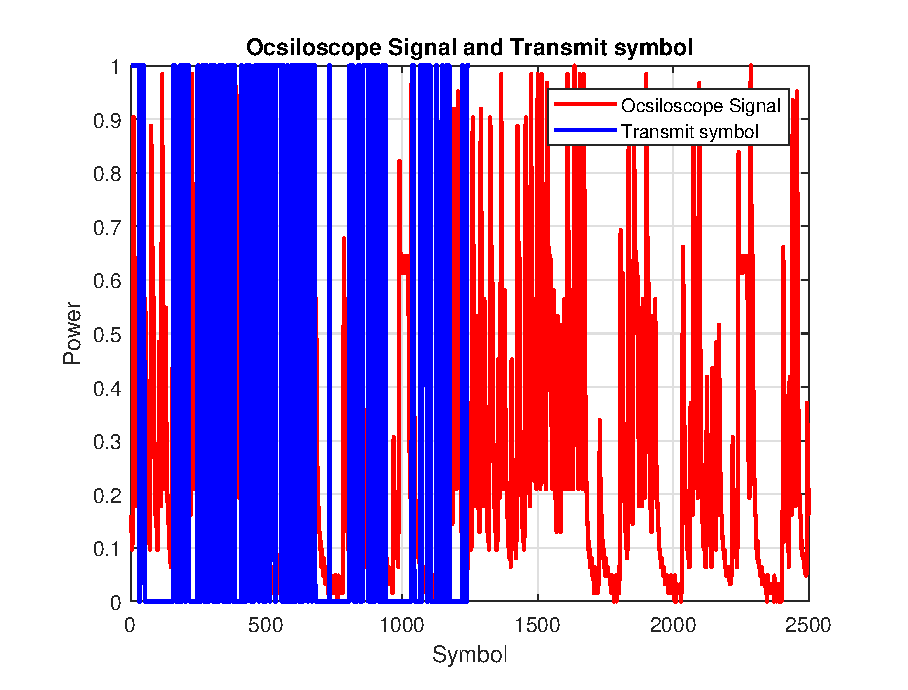
\includegraphics [scale=0.7]
	{ocsiloscope.eps}
	\caption{Tính độ tương quan giữa chuỗi phát và chuỗi thu}
	\label{fig:ocsiloscope}
\end{figure}
Dựa vào Hình \ref{fig:ocsiloscope}, ta có màu đỏ là tín hiệu sau khi thu đươc ocsiloscope đã chuẩn hóa công suất và màu xanh là tín hiệu truyền đi. Trong tín hiệu thu được ở ocsiloscope bao gồm tín hiệu truyền đi được lặp lại. Mục tiêu của chúng ta là xác định được điểm bắt đầu của tín hiệu và tách tín hiệu thu ứng với tín hiệu ta truyền đi. Ở đây ta có mỗi tín hiệu thu được là 2500 sample và cần ít nhất 2 tín hiệu truyền đi trên 1 tín hiệu thu để có thể tách được tín hiệu thu ứng với tín hiệu truyền. Trong báo cáo này chúng em chọn 5 sample và 250 symbol cho 1 tín hiệu.
Sau khi thu được tín hiệu. Dựa vào chuỗi truyền đi mà chúng ta tính độ tương quan bằng cách tính độ tương quan qua các lần dịch phải cho đến khi kết thúc tín hiệu thu. Kết quả sau khi tách chuỗi thu theo độ tương quan như Hình \ref{fig:ocsiloscope}.

\begin{figure}
	\centering
	\captionsetup{justification=centering}
	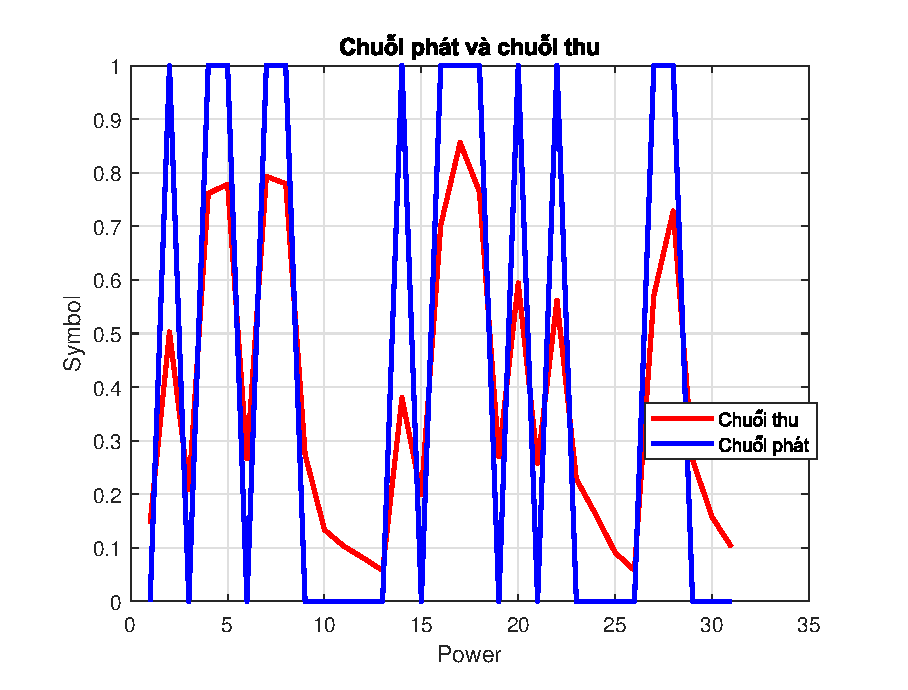
\includegraphics [scale=0.7]
	{transandreceive.eps}
	\caption{Độ tương quan giữa chuỗi phát và chuỗi thu}
	\label{fig:TransandReceive}
\end{figure}
\subsection{Ứng dụng mạng nơ-ron xác suất}
Trong đề tài luận văn này, tín hiệu được sử dụng là tín hiệu NRZ 2 mức 0 và 1,sau khi đi qua hệ thống sẽ bị biến đổi thành tín hiệu có các mức khác nhau. Bài toán đặt ra ở bộ cân bằng là làm thế nào để biến đổi các mức tín hiệu khác nhau về thành tín hiệu ban đầu có 2 mức 0 và 1. Để đánh giá tổng quan dữ liệu trước khi training có thể xem biểu đồ mắt như Hình \ref{fig:eye}.

\begin{figure}
	\centering
	\captionsetup{justification=centering}
	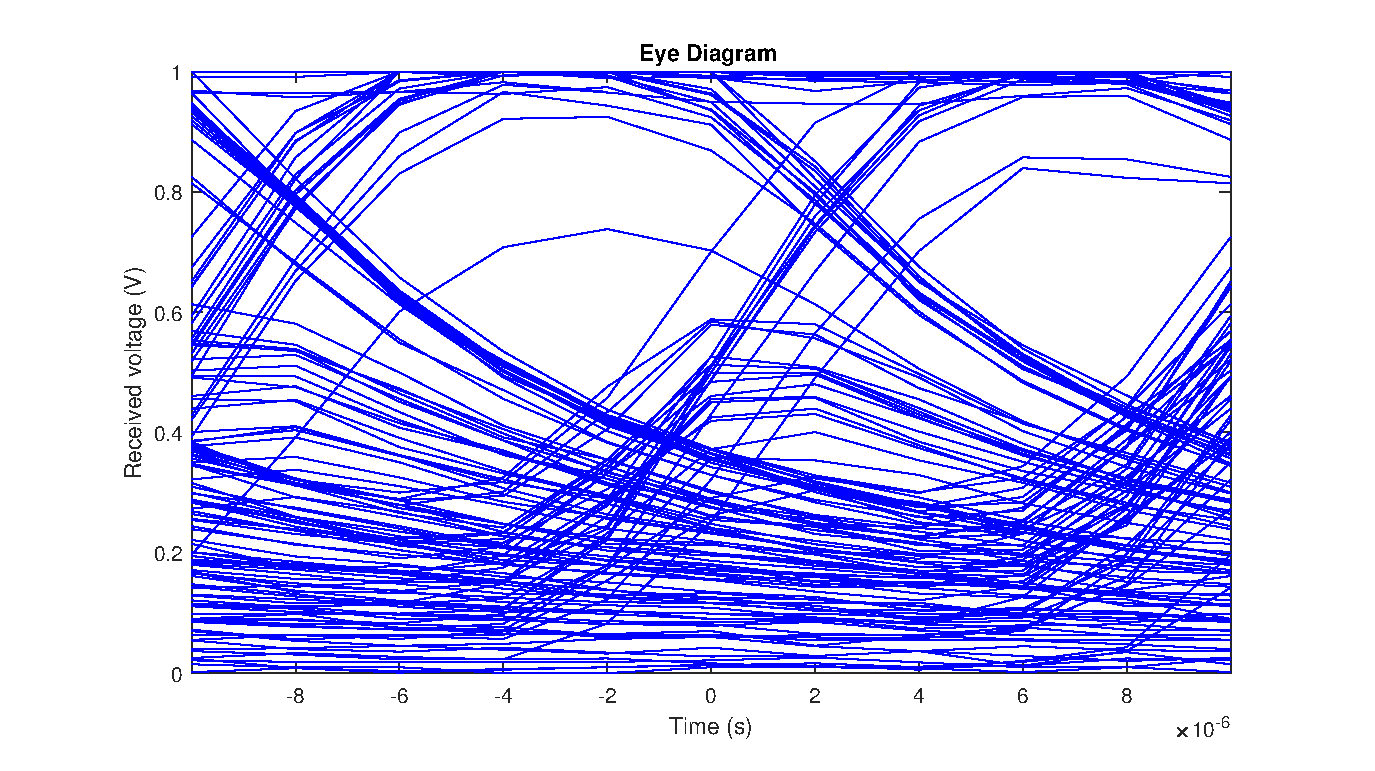
\includegraphics [scale=0.7]
	{eye.eps}
	\caption{Biểu đồ mắt}
	\label{fig:eye}
\end{figure}

Dựa vào \cite{eyediagram}, khi truyền ở tốc độ cao, chuỗi thu có gần như không xác định được độ mở mắt nên khó có thể phân loại được dữ liệu dựa vào mắt thường. Vì vậy mà chúng em quyết định bài toán phân lớp nên chúng em quyết định chọn mạng nơ-ron xác suất đề giải quyết vấn đề. Ngoài ra còn 1 điểm nữa là mô hình \ac{pnn} là 1 hàm có sẵn trong matlab mà còn rất tối ưu nên rất thuận tiện cho việc xử lý chuỗi tín hiệu lên đến hàng ngàn bit. Dựa vào chuỗi thu độ tương quan đã đề cập ở trên. Chúng ta chia nhỏ chuỗi thành các bit với nhãn '0' và '1' và tiến hành training bằng mạng nơ-ron xác suất. Từ đó đưa ra đánh giá đối với mô hình.


\newpage
\section{Kết quả và phân tích}
\subsection{Khảo sát sự ảnh hưởng của tốc độ bitrate}
Như đã đề cập, khi truyền ở tốc độ càng cao thì càng gây ra méo dạng phi tuyến. Mục tiêu trong khảo sát này là tìm ra được tốc độ truyền tối ưu có thể nhận biết được bằng mạng nơ-ron. Mục tiêu BER của khảo sát này là: 
 \begin{equation}
 	BER < 3.8*10^{-3}
 \end{equation}
Ta tiến hành khảo sát việc train và test dùng model PNN ở khoảng cách đo là 25cm ở các tốc độ bitrate: 40000,45000,50000,53000,55000,57000,60000,63000. Và xem xét sự thay đổi đổi BER. Từ đó ta có được đồ thị như Hình \ref{fig:BER}.

\begin{figure} [H]
	\centering
	\captionsetup{justification=centering}
	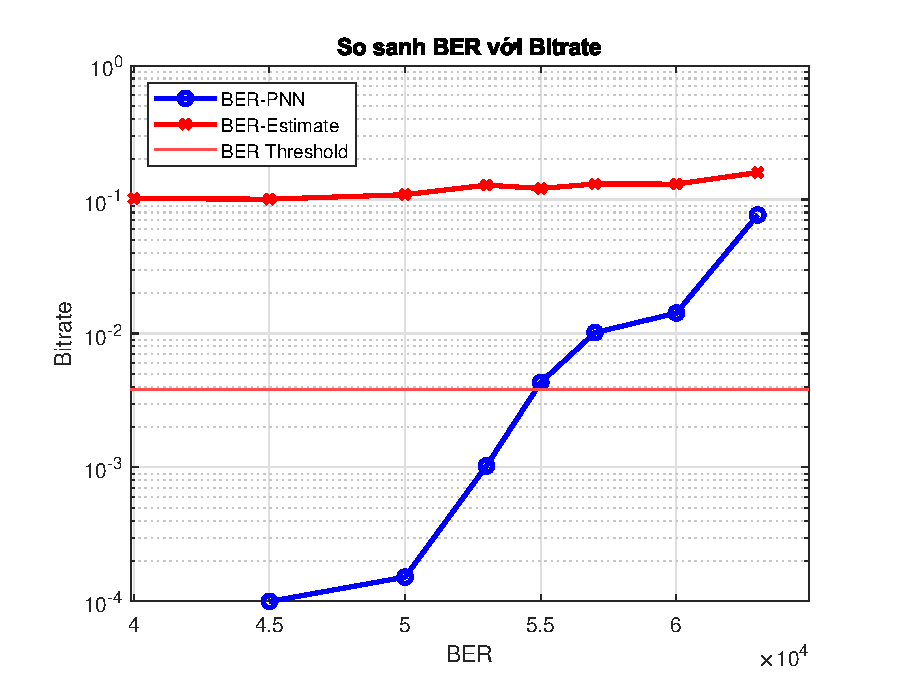
\includegraphics [scale=0.7]
	{BER.eps}
	\caption{So sánh BER giữa ước lượng và PNN}
	\label{fig:BER}
\end{figure}

Nhận xét: Từ đường màu đỏ có thể thấy BER mà chúng ta ước lượng dựa vào SNR gần như không đổi trên khoảng mà chúng ta khảo sát. Tuy nhiên khi sau khi sử dụng PNN thì giảm rõ rệt. Xét trên ngưỡng cắt BER thì ta có thể phân biệt được tín hiệu ở mức khoảng 54000.

\subsection{Khảo sát sự ảnh hưởng của số sample}
Xuất phát dựa trên việc cắt chuỗi các bit '0' và '1'. Việc tách chuỗi thu được tính dựa vào tương quan so với chuỗi phát. Việc lấy mẫu quá ít cũng có thể gây lệch chuỗi. Mục đích của khảo sát là tạo ra tập dữ liệu có độ tin cậy cao hơn để phân loại. Ngoài ra, việc tăng số sample có thể làm tăng số dữ liệu input. Việc này tuy làm chậm khả năng tính toán nhưng tăng tính ràng buộc của dữ liệu. Từ đó mà cho ta kết quả phân loại đúng hơn.





\chapter{Kết luận}

\section{Tóm tắt và kết luận chung}

Qua các số liệu cũng như các kết quả đã được đưa ra chương 3, chúng em có các kết luận sau:


\section{Hướng phát triển}

Một số hướng phát triển của đề tài:
\begin{itemize}
	\item nâng cấp mạch lái đèn led để hạn chế sự méo dạng cũng như xung cao để tránh làm hư đèn.
	\item Sử dụng tín hiệu lorentz sẽ tăng được tốc độ bit lên gấp 2-3 lần
	\item Tăng khoảng cách lên xa hơn để phù hợp với thực tế khác 
	\item Áp dụng các phương pháp neural network khác như generalized regression neural network, convolutionary neural network,...
\end{itemize}



%\bibliographystyle{reference/IEEEtran}
%\bibliography{IEEEabrv,reference/tailieuthamkhao}
\begin{thebibliography}{9}
	\bibitem{vlc} 
	Đặng Khánh Toàn, 
	\textit{Thiết kế bộ cân bằng cho hệ thống VLC sử dụng mạng nơ-ron tích chập}, 
	 Luận văn kỹ sư, Trường Đại Học Bách Khoa TP.HCM, tháng 9, 2020.
	
	\bibitem{askk} 
	Giới thiệu về giao thức ánh sáng khả kiến,
	\\\texttt{https://bkaii.com.vn/tin-tuc/225-gioi-thieu-ve-giao-thuc-anh-sang-kha-kien}
	
	\bibitem{bay} 
	Donald F.Specht, 
	\textit{Probabilistic Neural Networks}, 
	Lockheed Missiles and Space Company.Inc, 1990
	
	\bibitem{linecoding} 
	Nguyễn Ngọc Anh Khoa.
	\textit{Mô phỏng hệ thống MIMO VLC sử dụng NOMA-OFDM/FBMC}.
	Luận văn kĩ sư, Trường Đại Học Bách Khoa TP.HCM, tháng 12, 2017.
	
	\bibitem{pnn} 
	Probabilistic Neural Network by Wikipedia,
	\\\texttt{ https://en.wikipedia.org/wiki/Probabilistic-neural-network }
	
	\bibitem{2x2} 
	M.Kowalczyk.
	\textit{2x2 MIMO VLC Optical Transmission System Based on LEDs in a Double Role}.
	Warsaw University of Technology, Institute of Telecommunications, Warsaw, Poland.
	
\end{thebibliography}
\appendix
\titleformat{\chapter}
  {\Large\bfseries}
  {Phụ lục \thechapter .}
  {.5em}
  {\filleft\MakeUppercase}
  [\vspace{.5ex}]


\chapter{Code chương trình}

\section{Code tạo tín hiệu NRZ}

\lstinputlisting[language=Matlab, numbers=left, numberstyle=\small, breaklines]{code/creating_PAM_NRZ.m}

\section{Code lấy tín hiệu từ oscilloscope}

\lstinputlisting[language=Matlab, numbers=left, numberstyle=\small, breaklines]{code/Signal_oscilloscope.m}

\section{Code trích tín hiệu phát theo tín hiệu thu}

\lstinputlisting[language=Matlab, numbers=left, numberstyle=\small, breaklines]{code/Receiving_2.m}

\section{Code tính ước lượng SNR, BER}

\lstinputlisting[language=Matlab, numbers=left, numberstyle=\small, breaklines]{code/snrtruyenthong.m}

\section{Code tính BER theo PNN}

\lstinputlisting[language=Matlab, numbers=left, numberstyle=\small, breaklines]{code/pnn.m}






\end{document}